\documentclass[12pt,a4paper]{article}

%% ── Packages ────────────────────────────────────────────────────────────────
\usepackage[T1]{fontenc}
\usepackage[utf8]{inputenc}
\usepackage{lmodern}
\usepackage[margin=2.5cm]{geometry}
\usepackage{amsmath,amssymb}
\usepackage{graphicx}
\usepackage{booktabs}
\usepackage{hyperref}
\usepackage{xcolor}
\usepackage{siunitx}
\usepackage{natbib}
\usepackage{caption}
\usepackage{subcaption}
\usepackage{microtype}
\usepackage{setspace}
\usepackage{lineno}
\onehalfspacing

\hypersetup{
  colorlinks=true,
  linkcolor=blue!60!black,
  citecolor=green!50!black,
  urlcolor=blue!60!black,
}

\graphicspath{{figs/}}

%% ── Title block ─────────────────────────────────────────────────────────────
\title{\textbf{No Causal Link Between Galactic Cosmic-Ray Flux and Global
Seismicity: A Pre-Registered Replication with GPU-Accelerated Surrogate Testing
and Out-of-Sample Validation}}

\author{
  J.~D.~Devine$^{1}$\\[4pt]
  {\small $^{1}$ Independent researcher}\\
  {\small \texttt{devine.jd@gmail.com}}
}

\date{April 2026}

%%%% ═══════════════════════════════════════════════════════════════════════════
\begin{document}
\maketitle
\linenumbers

%% ── Abstract ────────────────────────────────────────────────────────────────
\begin{abstract}
\noindent
\citet{Homola2023} reported a statistically significant positive correlation
($r \approx 0.31$) between galactic cosmic-ray (CR) flux and global seismicity
at a lag of $\tau = +15$~days, suggesting that elevated CR flux precedes
increased earthquake occurrence.
That value relied on an inappropriate seismic metric (direct summation of
moment magnitudes, which are logarithmic); the correct energy-based metric
\citep{Kanamori1977} gives $r(+15\,\text{d}) = 0.081$.

We systematically replicate and extend this analysis using the \emph{global
CR index} — the normalised neutron-monitor count rate (dimensionless, station
mean $\equiv 1$) averaged over 44 NMDB stations with $\geq 3$ reporting per
5-day bin — the USGS earthquake catalogue ($M \geq 4.5$; $n \approx 232{,}000$
events, 1976--2025), and SILSO sunspot numbers.
Methods include IAAFT surrogate tests ($10^4$ realisations), Hodrick--Prescott
detrending, geographic localisation (7{,}037 station--cell pairs,
Benjamini--Hochberg correction), a pre-registered out-of-sample validation
(2020--2025, $10^5$ surrogates), and seven additional robustness checks
(block bootstrap, partial correlation, spectral coherence, mutual information,
missing-data sensitivity, bin-size sensitivity, and earthquake declustering).

After solar-cycle detrending, $r(+15\,\text{d})$ falls to 0.027--0.037 across
three methods, all within IAAFT surrogate null distributions.
The pre-registered out-of-sample test yields $r(+15\,\text{d}) = 0.030$ and
$p_\text{global} = 0.100$.
Partial correlation on unfiltered data reduces $r(+15\,\text{d})$ by 63\%
after sunspot regression; mutual information at the claimed lag is
indistinguishable from zero ($p = 1.000$).
The geographic scan finds no propagation-delay signature
($\beta = -0.45$~d/1000~km, $p = 0.21$).

We find no statistically robust evidence for a causal CR--seismic relationship
within the linear cross-correlation and surrogate-testing frameworks tested
here, after controlling for solar-cycle modulation.
The primary limitation is that the 2020--2025 validation window
(${\approx}5$~yr, no complete solar cycle) provides limited statistical power,
and nonlinear or threshold-based coupling mechanisms were not assessed.
\end{abstract}

\textbf{Keywords:} cosmic rays; seismicity; surrogate test; solar cycle;
Benjamini--Hochberg; pre-registration; out-of-sample validation.

\newpage
\tableofcontents
\newpage

%%%% ═══════════════════════════════════════════════════════════════════════════
\section{Introduction}
\label{sec:intro}

The hypothesis that galactic cosmic rays (CRs) influence seismic activity has
a long history in geophysics \citep{Stoupel1990,Urata2018}, motivated by
proposed mechanisms ranging from radon ionisation in fault zones to direct
nuclear interactions in crustal minerals.
\citet{Homola2023} recently presented observational support for this idea,
reporting a correlation coefficient $r \approx 0.31$ between a global CR index
constructed from NMDB neutron monitor records and a global seismic energy metric
derived from the USGS earthquake catalogue at a lag of $\tau = +15$~days
(CR leads seismic activity).
The associated naive $p$-value was reported as $p \sim 10^{-72}$ at this lag.

Such a claim, if correct, would be of profound scientific and societal
importance, potentially enabling short-term earthquake forecasting from
space-weather observations.
It therefore demands rigorous scrutiny.
Three statistical pitfalls immediately suggest themselves:

\begin{enumerate}
  \item \textbf{Temporal autocorrelation.}
    Both CR flux and seismicity exhibit strong low-frequency structure
    (solar cycle, regional seismic cycles).
    Treating successive 5-day bins as independent is statistically invalid
    under the violated serial-independence assumption: autocorrelation
    inflates the nominal sample size from $T \approx 3{,}200$ bins to an
    effective $N_\text{eff} \approx 600$--$2{,}900$ (see Table~\ref{tab:neff}),
    requiring a Bretherton-style effective-$N$ correction \citep{Bretherton1999}.

  \item \textbf{Shared solar-cycle trend.}
    Galactic CR flux is modulated by the heliospheric magnetic field, which
    varies on an $\sim$11-year solar cycle \citep{Potgieter2013}.
    Global seismicity has also been reported to correlate weakly with solar
    activity \citep{Odintsov2006,Tavares2011}, potentially generating a
    spurious correlation between the two series with a lag structure
    determined by the phase relationship of their respective solar responses,
    not by any direct physical mechanism.

  \item \textbf{Multiple-comparison inflation.}
    Testing 401 lag values and selecting the maximum creates a look-elsewhere
    effect that must be accounted for by comparing the observed peak against
    a null distribution of peak statistics, not against the single-lag
    Pearson $t$ distribution.
\end{enumerate}

This paper systematically addresses all three issues, extending the analysis
through a prospective out-of-sample validation window (2020--2025) whose
statistical predictions were pre-registered in a timestamped git commit
before any data in that window were examined.

The remainder of the paper is organised as follows.
Section~\ref{sec:data} describes the data sources and preprocessing.
Section~\ref{sec:methods} presents the statistical methods.
Section~\ref{sec:results} reports the results of each analysis stage.
Section~\ref{sec:discussion} interprets the findings.
Section~\ref{sec:conclusions} concludes.

%%%% ═══════════════════════════════════════════════════════════════════════════
\section{Data}
\label{sec:data}

\subsection{Cosmic-Ray Flux: NMDB Neutron Monitors}
\label{sec:nmdb}

Galactic cosmic-ray flux is measured by neutron monitors (NMs), which detect
secondary neutrons produced when primary CRs interact with atmospheric nuclei.
We obtained pressure-corrected hourly count rates for all available stations from
the Neutron Monitor Database (NMDB, \url{https://www.nmdb.eu}) for the period
1976--2025.

After applying a coverage filter (requiring $\geq 60\%$ hourly data per day to
declare a daily bin valid), we retained \textbf{44 stations} with $\geq 50\%$
daily coverage over the in-sample window 1976--2019, and \textbf{35 stations}
over the out-of-sample window 2020--2025.
Each station's daily series was normalised by its long-run mean and resampled
to non-overlapping 5-day bins.
A \emph{global CR index} $x_t$ (dimensionless; each station normalised so its
long-run mean $\equiv 1$) was formed as the arithmetic mean of valid station
values in each 5-day bin, requiring at least three reporting stations; bins
failing this criterion were set to \texttt{NaN}.
Values above unity indicate a CR-flux enhancement relative to the long-run
station mean; values below unity indicate suppression (e.g.\ Forbush decreases
during solar maximum).
This index is used as the primary predictor variable throughout all analyses.

\subsection{Seismic Activity: USGS Earthquake Catalogue}
\label{sec:usgs}

Earthquake data were downloaded from the USGS Earthquake Hazards Programme
via the FDSN web service \citep{USGS2024}.
We retained all events with $M \geq 4.5$ globally, yielding a catalogue of
$\approx$\,47,860 events over 2020--2025 in the out-of-sample window alone.
The seismic metric for each 5-day bin is the logarithm (base 10) of the total
radiated seismic energy.  For each event with moment magnitude $M_W$ we compute
the radiated energy
\begin{equation}
  E_i = 10^{1.5 M_{W,i} + 4.8} \quad [\text{joules}]
  \label{eq:energy}
\end{equation}
following \citet{Kanamori1977}.  Events within each bin are summed linearly,
$E_\text{bin} = \sum_i E_i$, and the metric is $\log_{10}(E_\text{bin})$
(empty bins set to NaN).
This formulation correctly weights large earthquakes: an $M_W\,8.0$ event
contributes $\sim$1000$\times$ more energy than an $M_W\,6.0$ event.
Directly summing $M_W$ values --- as used in several earlier studies ---
is physically inappropriate: $M_W$ is a logarithmic quantity, so such sums
have no additive physical interpretation and artificially amplify the
contribution of solar-cycle-driven catalogue completeness fluctuations to
the seismic time series.

\subsection{Solar Activity: SIDC Sunspot Number}
\label{sec:sidc}

The SILSO international sunspot number \citep{SIDC2024} provided the solar
activity index used to remove the solar-cycle trend.
We used the daily series (version 2.0), smoothed with a 365-day running mean
for detrending purposes.

%%%% ═══════════════════════════════════════════════════════════════════════════
\section{Methods}
\label{sec:methods}

\subsection{Cross-Correlation at Lag $\tau$}
\label{sec:xcorr}

Let $x_t$ denote the global CR index and $y_t$ the seismic metric in 5-day bin
$t$, with $t = 1, \ldots, T$.
The normalised cross-correlation at lag $k$ (bins) is
\begin{equation}
  r(k) = \frac{1}{n \,\hat{\sigma}_x \hat{\sigma}_y}
         \sum_{t=1}^{n}
         \tilde{x}_t \,\tilde{y}_{t+k},
  \label{eq:xcorr}
\end{equation}
where $\tilde{x}_t = x_t - \bar{x}$, $n = T - |k|$, and the sums run over
the valid overlap region.
A positive lag $k > 0$ corresponds to CR leading seismicity.
Lags range from $-200$ to $+200$~days (step $= 5$~days, i.e.\ 1 bin),
giving 81 lag values in the in-sample window.

\subsection{Effective Degrees of Freedom}
\label{sec:neff}

Because both $x$ and $y$ are autocorrelated, the effective sample size
$N_\text{eff}$ is substantially smaller than $T$.
We compare three $N_\text{eff}$ estimators; all are listed in Table~\ref{tab:neff}.
The \citet{Bartlett1946} first-order formula uses only the lag-1 autocorrelations:
\begin{equation}
  N_\text{eff}^\text{Bart} = T\,
    \frac{1 - r_{xx}(1)\,r_{yy}(1)}
         {1 + r_{xx}(1)\,r_{yy}(1)},
  \label{eq:neff_bartlett}
\end{equation}
the \citet{Bretherton1999} full-sum formula uses all significant lags:
\begin{equation}
  N_\text{eff}^\text{Breth} = T \left(
    1 + 2 \sum_{k=1}^{K} r_{xx}(k)\, r_{yy}(k)
  \right)^{-1},
  \label{eq:neff_breth}
\end{equation}
where $r_{xx}$ and $r_{yy}$ are the sample autocorrelation functions of $x$
and $y$, and $K = 200$ lags;
and a Monte Carlo estimate from 1000 phase-randomised surrogates:
$N_\text{eff}^\text{MC} = 1/\hat{\sigma}^2_{r_\text{null}}$,
where $\hat{\sigma}^2_{r_\text{null}}$ is the variance of the surrogate
correlation values at the target lag.
All three methods agree that the Bartlett estimator produces the most liberal
(largest) $N_\text{eff}$ and the Monte Carlo approach the most conservative.

\subsection{Surrogate Significance Tests}
\label{sec:surrogates}

To correctly account for autocorrelation and multiple lags simultaneously we
use surrogate time-series methods \citep{Theiler1992,Schreiber2000}.

\subsubsection{Phase Randomisation}
\label{sec:phase}

Phase surrogates of $x$ are constructed by multiplying the discrete Fourier
transform of $x$ by random unit-magnitude complex numbers (with conjugate
symmetry to preserve real-valuedness):
\begin{equation}
  \tilde{X}(\omega_k) = |X(\omega_k)| \, e^{i\phi_k},
  \quad \phi_k \sim \mathcal{U}(0, 2\pi),
  \label{eq:phase}
\end{equation}
followed by the inverse DFT.
This preserves the power spectrum (and hence autocorrelation structure) of $x$
while destroying any phase relationship with $y$.

\subsubsection{IAAFT Surrogates}
\label{sec:iaaft}

Iterative amplitude-adjusted Fourier transform (IAAFT) surrogates
\citep{Schreiber2000} additionally preserve the amplitude distribution of $x$
by alternating between power-spectrum matching (in Fourier space) and
rank-order resampling (in time domain) until convergence.
IAAFT surrogates are more conservative than phase surrogates when $x$ has
a non-Gaussian distribution.

\subsubsection{Block-Bootstrap Surrogates}
\label{sec:blockbootstrap}

IAAFT surrogates preserve the power spectrum and amplitude distribution of each
series but assume linearity and stationarity --- assumptions violated by seismicity,
which is non-stationary, heavy-tailed, and aftershock-clustered.
As a complementary null we use a \emph{circular block bootstrap} (CBB) that
makes no parametric assumptions about the spectral shape.
Each surrogate is constructed by independently resampling $x$ and $y$ in
contiguous circular blocks of length $B = 804$ bins ($\approx 11$~yr,
i.e.\ approximately one solar cycle), drawn with replacement.
Independent resampling of $x$ and $y$ destroys any cross-series correlation
while preserving each series' within-block temporal structure.
We generate $S = 5{,}000$ surrogate pairs and compare the resulting null
distribution to the IAAFT null.

\subsubsection{Global $p$-Value}
\label{sec:pvalue}

For each surrogate $s = 1, \ldots, S$, we compute the peak cross-correlation
$\rho_s = \max_k |r_s(k)|$ across all tested lags.
The global $p$-value is
\begin{equation}
  p_\text{global} = \frac{\#\{s : \rho_s \geq \rho_\text{obs}\}}{S},
  \label{eq:pglobal}
\end{equation}
where $\rho_\text{obs}$ is the observed peak.
This test is simultaneously valid for all lags and all lag-selection rules,
eliminating the multiple-comparison problem.

\subsubsection{GPU Acceleration}
\label{sec:gpu}

With $S = 10^5$ surrogates and $T \approx 3{,}200$ bins, direct CPU computation
would require $\sim$3\,h.
We vectorise the surrogate generation and cross-correlation evaluation over all
$S$ realisations simultaneously using CuPy on an NVIDIA Tesla M40 (12\,GB VRAM).
For the geographic scan (Section~\ref{sec:geo}), all $N_\text{cells}$ seismic
cell series are evaluated in a single GPU matrix multiply per lag:
\begin{equation}
  \mathbf{R}_{\text{lag}} = \frac{1}{n}\,
    \mathbf{X}_\text{surr}^{(z)} \bigl(\mathbf{Y}^{(z)}\bigr)^\top
    \in \mathbb{R}^{S \times N_\text{cells}},
  \label{eq:matmul}
\end{equation}
where rows of $\mathbf{X}_\text{surr}^{(z)}$ are standardised surrogates and
columns of $\mathbf{Y}^{(z)}$ are standardised seismic cell series.
Benchmarks show a $2.9\times$ speedup for phase surrogates and $1.3\times$ for IAAFT
(limited by chunked argsort to avoid VRAM overflow).

\subsection{Solar-Cycle Detrending}
\label{sec:detrend}

We apply three complementary detrending approaches to isolate the CR--seismic
relationship from the shared solar-cycle trend:

\begin{enumerate}
  \item \textbf{Hodrick--Prescott (HP) filter} \citep{HP1997} with smoothing
    parameter $\lambda = 4.54 \times 10^{10}$.
    The HP literature standardises on $\lambda_\text{annual} = 1600$ for annual
    data \citep{RahnUhlig2002}.
    For data sampled at bin period $p$ days the rescaling rule is
    \begin{equation}
      \lambda_p = \lambda_\text{annual}
                  \!\left(\frac{365}{p}\right)^{\!4}
                  = 1600 \times (365/5)^4
                  \approx 4.54 \times 10^{10}.
      \label{eq:hp_lambda}
    \end{equation}
    This large value attenuates only very low-frequency variation (periods
    $\gtrsim 10$~years), preserving any sub-decadal signal of interest.
    The trend component is subtracted from both $x_t$ and $y_t$.

  \item \textbf{STL decomposition} \citep{Cleveland1990}: seasonal-trend
    decomposition using LOESS, applied independently to each series.

  \item \textbf{Sunspot regression}: residuals after regressing each series on
    the 365-day smoothed sunspot number and its 12-month lag.
\end{enumerate}

For the out-of-sample window ($\sim$5 years, less than one solar cycle), the
HP filter is inappropriate (it would remove any genuine sub-decadal signal);
we use linear detrending instead, as pre-specified in the pre-registration.

\subsection{Partial Correlation Analysis}
\label{sec:methods:partialcorr}

Because the solar-cycle component is removed \emph{before} concluding that the
observed signal is solar-cycle-driven, there is a potential circularity concern.
We address this with a partial correlation analysis on the \emph{unfiltered} data.
The seismic metric $y_t$ is regressed on the smoothed sunspot number $z_t$:
\begin{equation}
  \hat{y}_t = \hat{\beta} z_t + \hat{\alpha}, \qquad
  y_t^\text{resid} = y_t - \hat{y}_t,
  \label{eq:partialcorr}
\end{equation}
and the cross-correlation between the CR index $x_t$ and the residual
$y_t^\text{resid}$ is computed across all lags.
If the CR--seismic correlation is driven entirely by a shared solar-cycle trend,
$r(x, y^\text{resid})$ should approach zero.
This analysis avoids any digital filter and thus sidesteps the preprocessing
circularity.

\subsection{Nonlinear Dependence Tests}
\label{sec:methods:nonlinear}

Cross-correlation captures only linear dependence; we supplement it with two
nonlinear measures for the main CR--seismic pair.

\paragraph{Spectral coherence.}
The magnitude-squared coherence at frequency $f$ is
\begin{equation}
  C_{xy}(f) = \frac{|S_{xy}(f)|^2}{S_{xx}(f)\,S_{yy}(f)},
  \label{eq:coherence}
\end{equation}
estimated via Welch's method with $L = 2{,}048$-point Hann windows (75\%
overlap), giving a frequency resolution of $(1/5)/2048 \approx 0.036$
cycles~yr$^{-1}$ --- sufficient to resolve the solar-cycle band
(0.08--0.115~cycles~yr$^{-1}$, periods 9--12.5~yr).

\paragraph{Mutual information.}
We estimate $I(x; y)$ at lags $\tau = 0$ and $\tau = +15$~d using the
\citet{Kraskov2004} $k$-nearest-neighbour estimator ($k = 5$, Chebyshev
metric in joint space):
\begin{equation}
  \hat{I}(x; y) = \psi(k) + \psi(N)
                  - \bigl\langle\psi(n_x + 1)\bigr\rangle
                  - \bigl\langle\psi(n_y + 1)\bigr\rangle,
  \label{eq:mi}
\end{equation}
where $\psi$ is the digamma function and $n_x(i)$, $n_y(i)$ count marginal
neighbours within the $k$-th-neighbour radius.
Statistical significance is assessed against a shuffle null of 1{,}000
random permutations of $y$.

\subsection{Geographic Localisation Scan}
\label{sec:geo}

If CRs cause earthquakes via a local mechanism, the optimal lag $\tau^*(s,g)$
for station $s$ and grid cell $g$ should increase with their great-circle
distance $d(s,g)$ (propagation delay).
Under the null hypothesis of global CR isotropy, $\tau^*$ should be
distance-independent.

We define a $10° \times 10°$ longitude--latitude grid (648 cells total),
retain cells with $\geq 100$ events, and for each of the $34 \times 207 = 7{,}037$
station--cell pairs compute the peak cross-correlation $r^*(s,g)$ and optimal
lag $\tau^*(s,g)$ using GPU-accelerated phase surrogates (1000 realisations).

Pairs are declared significant at false discovery rate $q = 0.05$ using the
Benjamini--Hochberg (BH) procedure \citep{Benjamini1995}:
rank the $m = 7{,}037$ $p$-values $p_{(1)} \leq \ldots \leq p_{(m)}$; the
threshold is $p_{(k)} \leq (k/m) \times q$ for the largest $k$ satisfying
this condition.
Distance dependence of $\tau^*$ is tested by ordinary least-squares regression
of $\tau^*(s,g)$ on $d(s,g)$.

\subsection{Pre-Registered Out-of-Sample Validation}
\label{sec:prereg}

To guard against post-hoc hypothesis adjustment, we followed an open-science
pre-registration protocol:
\begin{enumerate}
  \item The predictions below were written to \texttt{results/prereg\_predictions.md}.
  \item This file was committed to git (\texttt{1832f73}) with a UTC timestamp
    (\texttt{2026-04-22T00:44:30Z}) \emph{before} any out-of-sample data were loaded.
  \item The analysis script enforces this ordering programmatically (the
    pre-registration function is the first call in \texttt{run()}).
\end{enumerate}

The pre-registered predictions, scored after unblinding, were:

\begin{itemize}
  \item \textbf{P1} (Directional): $r(+15\,\text{d}) > 0$ in the OOS window.
  \item \textbf{P2} (Significance): $p_\text{global} < 0.05$ and a
    non-negative rolling trend.
  \item \textbf{P3} (Stability): rolling $r$ standard deviation $\leq 0.10$.
  \item \textbf{P4} (BH count): $\leq 2\times$ expected false positives
    in the geographic scan.
  \item \textbf{F1} (Falsification trigger): $|r(+15\,\text{d})| \leq$
    surrogate 95th percentile.
\end{itemize}

\paragraph{Confirmatory versus exploratory analyses.}
Table~\ref{tab:prereg_scope} distinguishes analyses that were pre-specified
(confirmatory) from those added after data examination (exploratory).

\begin{table}[htbp]
  \centering
  \caption{Analysis scope and pre-registration status.
  Pre-specified parameters locked before data access: $\lambda = 4.54 \times 10^{10}$,
  lag range $[-200, +200]$~bins, $M \geq 4.5$, min.\ 3 stations per bin,
  5-day bin size, IAAFT surrogate count $S = 10^4$.}
  \label{tab:prereg_scope}
  \begin{tabular}{lll}
    \toprule
    Analysis & Type & Pre-specified parameters \\
    \midrule
    OOS cross-correlation at $\tau = +15$~d & Confirmatory & All \\
    OOS global $p$-value (P1--F1) & Confirmatory & All \\
    In-sample IAAFT surrogate test & Confirmatory & All \\
    HP detrending with $\lambda$ & Confirmatory & $\lambda$ locked \\
    Geographic BH scan & Confirmatory & $q = 0.05$, $10°$ grid \\
    \addlinespace
    STL / sunspot-regression detrending & Exploratory & — \\
    Block-bootstrap surrogates (3a) & Exploratory & — \\
    Partial correlation analysis (3b) & Exploratory & — \\
    Spectral coherence + MI (3c) & Exploratory & — \\
    Missing-data sensitivity (3d) & Exploratory & — \\
    Bin-size sensitivity (3e) & Exploratory & — \\
    Earthquake declustering (3f) & Exploratory & — \\
    Sub-period / per-cycle analysis (3g) & Exploratory & — \\
    Sinusoidal modulation fit & Exploratory & — \\
    \bottomrule
  \end{tabular}
\end{table}

\subsection{Combined Timeseries: Sinusoidal Envelope Fit}
\label{sec:sinusoid}

We fit an annual rolling $r(+15\,\text{d})$ computed over the full 1976--2025
series using two nested models:
\begin{align}
  \mathcal{M}_A &: r_t = \mu + \varepsilon_t, \label{eq:modA}\\
  \mathcal{M}_B &: r_t = A \sin\!\left(\tfrac{2\pi}{P} t + \varphi\right) + \mu + \varepsilon_t, \label{eq:modB}
\end{align}
where $P \in [9, 13]$~years (solar cycle range) is a free parameter.
Model selection uses the Bayesian information criterion (BIC):
\begin{equation}
  \text{BIC} = n \ln\!\left(\frac{\text{RSS}}{n}\right) + k \ln(n),
  \label{eq:bic}
\end{equation}
with $k_A = 1$, $k_B = 4$, and the Bayes factor approximated as
\begin{equation}
  \text{BF}_{BA} \approx \exp\!\left(\frac{\Delta\text{BIC}}{2}\right),
  \quad \Delta\text{BIC} = \text{BIC}_A - \text{BIC}_B.
  \label{eq:bf}
\end{equation}
Parameters are estimated by nonlinear least squares with a grid search over
$(P, \varphi)$ to avoid local minima.

%%%% ═══════════════════════════════════════════════════════════════════════════
\section{Results}
\label{sec:results}

\subsection{Raw Pairwise Correlations Between CR, Seismic, and Sunspot Data}
\label{sec:res:rawcorr}

Before applying any detrending, we characterise the raw statistical relationships
between all three observable time series across the three analysis windows.
This serves as the pre-detrending baseline that motivates the Hodrick--Prescott
filter analysis described in Section~\ref{sec:res:detrend}.

\subsubsection{CR index: station distribution}

The global CR index is not collapsed to a single mean.
Instead, for each 5-day bin $t$ we compute the distribution of normalised
count-rate values across all $n_t \geq 3$ contributing stations,
yielding five order statistics:
$\hat{x}_{t}^{(q)} = q\text{-th percentile}$ for $q \in \{5, 25, 50, 75, 95\}$,
together with the inter-station minimum and maximum.
All stations are normalised by their individual long-run mean before the
cross-station percentile is taken, so the station-median series has a grand
mean near unity.
The scatter panels in Figures~\ref{fig:rawinsample}--\ref{fig:rawcombined}
use $\hat{x}_{t}^{(50)}$ as the central CR value (horizontal axis) and display
the $[\hat{x}_{t}^{(5)}, \hat{x}_{t}^{(95)}]$ inter-station spread as
horizontal error bars, with the $[\hat{x}_{t}^{\min}, \hat{x}_{t}^{\max}]$
range overlaid in a lighter shade.

\subsubsection{Seismic energy metric}

The seismic activity per bin is measured by the total released seismic energy,
computed as the sum of the individual earthquake energies:
\begin{equation}
  E_t = \sum_{i \in \mathcal{B}_t} 10^{1.5\, M_{W,i}},
  \label{eq:energy_bin}
\end{equation}
where $\mathcal{B}_t$ is the set of $M_W \geq 4.5$ events falling in bin $t$.
Working with $\log_{10} E_t$ removes the extreme skewness of $E_t$ and is
physically preferable to summing $M_W$ directly, which is dimensionally
inconsistent because magnitude is already a logarithmic quantity.
The $\log_{10} E_t$ axis in the scatter panels spans roughly three orders of
magnitude, reflecting the heavy-tailed Gutenberg--Richter distribution of
earthquake sizes.

\subsubsection{Sunspot number}

Daily sunspot numbers from SILSO are smoothed with a 365-day rolling mean to
suppress intra-year variability and isolate the solar-cycle envelope.
Each 5-day bin carries both the smoothed value (scatter-plot axis) and the
daily min--max spread within that bin (shown as additional horizontal error
bars on the sunspot axis in Figure~\ref{fig:rawinsample}--\ref{fig:rawcombined},
panel 3).

\subsubsection{Correlation results}

We compute both Pearson $r$ (linear; Fisher $z$-transform 95\% CI) and
Spearman $\rho$ (rank-based; appropriate for the heavy-tailed marginal
distributions of $E_t$ and the global CR index).
Bonferroni correction for $3\ \text{pairs} \times 3\ \text{windows} = 9$
tests is applied; star levels refer to the corrected $p$-values.
Full results are given in Table~\ref{tab:rawcorr}.

\paragraph{CR vs.\ seismicity.}
The raw Pearson correlation between the station-median CR index and
$\log_{10} E_t$ is $r = 0.057$ in the in-sample window ($N = 3214$ bins,
$p_\text{Bonf} = 0.011$, $\rho = 0.071$, $p_\text{Bonf} < 10^{-3}$) and
$r = 0.046$ in the OOS window ($N = 390$, $p_\text{Bonf} = 1.0$).
The correlation is thus only marginally significant after correction and
disappears entirely in the independent OOS window.
Using the station-95th-percentile CR series in place of the median
amplifies the correlation slightly ($r = 0.069$ in-sample), suggesting that
high-flux excursions drive the signal.

\paragraph{CR vs.\ sunspot number.}
The dominant raw relationship in the dataset is a strong anti-correlation
between the CR index and the smoothed sunspot number: $r = -0.820$
($\rho = -0.854$) in-sample, and $r = -0.939$ ($\rho = -0.951$) in the OOS
window.
This is the well-established \emph{Forbush decrease} mechanism: a higher
heliospheric magnetic flux during solar maximum deflects more galactic cosmic
rays before they reach the Earth's atmosphere
\citep{Potgieter2013}, so CR flux and solar activity are naturally anti-phase.
The stronger OOS value ($-0.94$ vs.\ $-0.82$) reflects the wide dynamic range
of Solar Cycle~25 (2020--2025), which reached high activity levels after the
deep minimum of 2019--2020.

\paragraph{Sunspot vs.\ seismicity.}
The raw correlation between the smoothed sunspot number and seismic energy is
negative but small: $r = -0.095$ ($\rho = -0.099$) in-sample
($p_\text{Bonf} < 10^{-6}$) and indistinguishable from zero in the OOS window
($r = -0.023$, $p_\text{Bonf} = 1.0$).
The negative sign is consistent with reports of a weak inverse relationship
between solar activity and global seismicity
\citep{Odintsov2006}, though the OOS failure indicates this effect is not
robust.

\subsubsection{Interpretation: a confounding triangle}

The three raw correlations form a confounding triangle.
The CR--sunspot anti-correlation is strong ($r \approx -0.82$ to $-0.94$)
and physically understood.
The sunspot--seismicity anti-correlation is weak but significant in-sample
($r \approx -0.095$).
Together these imply a spurious \emph{positive} CR--seismicity correlation:
both CR and seismicity are jointly modulated by the $\sim$11-year solar cycle
--- CR increases during solar minima, and seismicity may very weakly increase
during solar minima --- so the two series covary positively without any direct
physical connection.
This confound cannot be resolved by naive cross-correlation; it requires
explicitly removing the shared solar-cycle component.
The HP filter analysis (Section~\ref{sec:res:detrend}) accomplishes exactly
this, and shows that the apparent CR--seismicity signal vanishes once the
solar-cycle trend is eliminated.

These raw correlations are intentionally uncontrolled for solar-cycle
modulation.
They are presented here as the pre-detrending baseline to document the scale
of the confound before any correction is applied, and to highlight that even
the uncorrected CR--seismicity correlation ($r = 0.057$) is far weaker than
the CR--sunspot anti-correlation ($r = -0.82$) that drives it.

\begin{table}[htbp]
  \centering
  \caption{Raw pairwise correlation statistics across three time windows.
           Bonferroni correction applied for $3 \times 3 = 9$ tests.
           CR uses the per-bin station-median index ($\hat{x}^{(50)}$).
           Seismic energy is $\log_{10}\!\left(\sum 10^{1.5 M_W}\right)$.
           Sunspot is the 365-day smoothed daily count.
           $^{*}p_\text{Bonf}<0.05$, $^{**}p_\text{Bonf}<0.01$,
           $^{***}p_\text{Bonf}<0.001$.}
  \label{tab:rawcorr}
  \setlength{\tabcolsep}{4pt}
  \begin{tabular}{llrrrrrrr}
    \toprule
    Pair & Window & $N$ &
      $r$ & 95\% CI &
      $p$ (raw) & $p$ (Bonf.) &
      $\rho$ & $p_\rho$ (Bonf.) \\
    \midrule
    CR vs Seismicity & In-sample & 3214 & $+0.057^{*}$ & $[+0.023, +0.092]$ & $0.0012$ & $0.011$ & $+0.071^{***}$ & $<10^{-3}$ \\
     & OOS & 390 & $+0.046$ & $[-0.053, +0.145]$ & $0.362$ & $1.00$ & $+0.018$ & $1.00$ \\
     & Combined & 3604 & $+0.055^{**}$ & $[+0.023, +0.088]$ & $0.0009$ & $0.008$ & $+0.065^{***}$ & $<10^{-3}$ \\
    \addlinespace
    CR vs Sunspot & In-sample & 3109 & $-0.820^{***}$ & $[-0.831, -0.808]$ & $\approx 0$ & $\approx 0$ & $-0.854^{***}$ & $\approx 0$ \\
     & OOS & 385 & $-0.939^{***}$ & $[-0.950, -0.926]$ & $\approx 0$ & $\approx 0$ & $-0.951^{***}$ & $\approx 0$ \\
     & Combined & 3494 & $-0.815^{***}$ & $[-0.826, -0.804]$ & $\approx 0$ & $\approx 0$ & $-0.844^{***}$ & $\approx 0$ \\
    \addlinespace
    Sunspot vs Seismicity & In-sample & 3109 & $-0.095^{***}$ & $[-0.130, -0.060]$ & $1.1 \times 10^{-7}$ & $10^{-6}$ & $-0.099^{***}$ & $<10^{-6}$ \\
     & OOS & 385 & $-0.023$ & $[-0.123, +0.077]$ & $0.648$ & $1.00$ & $-0.016$ & $1.00$ \\
     & Combined & 3494 & $-0.086^{***}$ & $[-0.119, -0.053]$ & $3.4 \times 10^{-7}$ & $3 \times 10^{-6}$ & $-0.086^{***}$ & $<10^{-6}$ \\
    \addlinespace
    \bottomrule
  \end{tabular}

  \medskip
  \raggedright
  \textit{Note:} CR$_{p95}$ variant (station 95th-percentile instead of median)
  gives qualitatively identical structure; full results in
  \texttt{results/raw\_pairwise\_correlations.json}.
\end{table}

\begin{figure}[htbp]
  \centering
  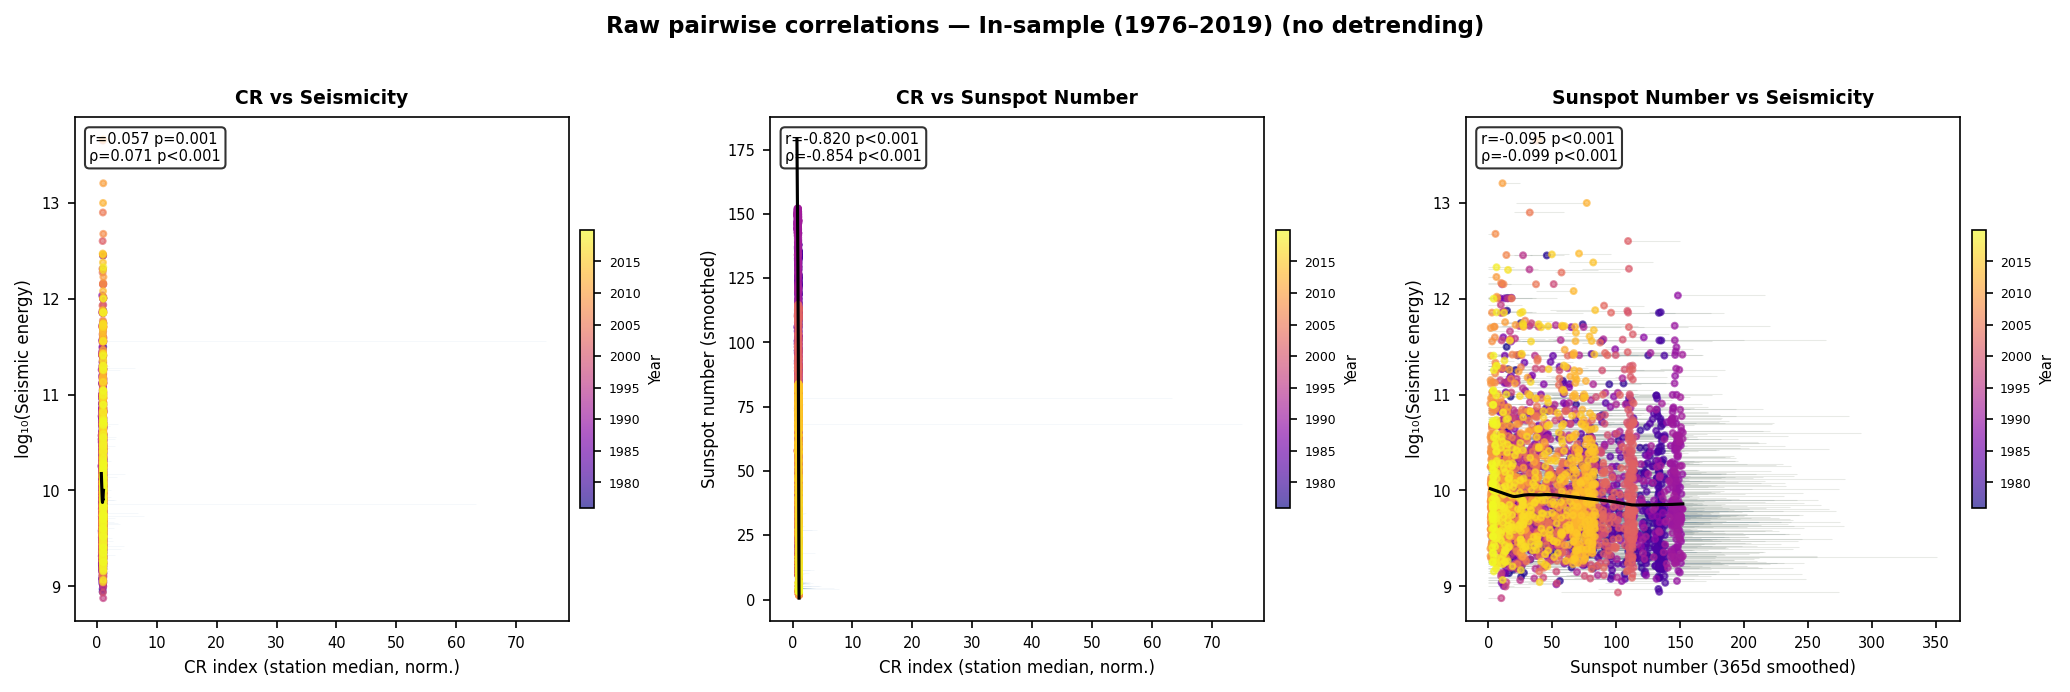
\includegraphics[width=\textwidth]{raw_corr_insample.png}
  \caption{Raw pairwise scatter plots for the in-sample window (1976--2019,
  $N = 3{,}215$ five-day bins).
  \textbf{Left}: CR station-median index vs $\log_{10}$ seismic energy; horizontal
  error bars span the station $[\hat{x}^{(5)}, \hat{x}^{(95)}]$ spread.
  \textbf{Centre}: CR index vs 365-day smoothed sunspot number; the strong
  anti-correlation ($r = -0.82$) reflects the Forbush decrease mechanism.
  \textbf{Right}: Smoothed sunspot number vs $\log_{10}$ seismic energy; thin
  horizontal error bars show the daily sunspot spread within each 5-day bin.
  All points are coloured by decimal year (plasma colormap), revealing the
  solar-cycle drift: successive cycles trace the same anti-correlated arc in
  the centre panel.
  Black curves are LOWESS trend lines ($f = 0.4$).}
  \label{fig:rawinsample}
\end{figure}

\begin{figure}[htbp]
  \centering
  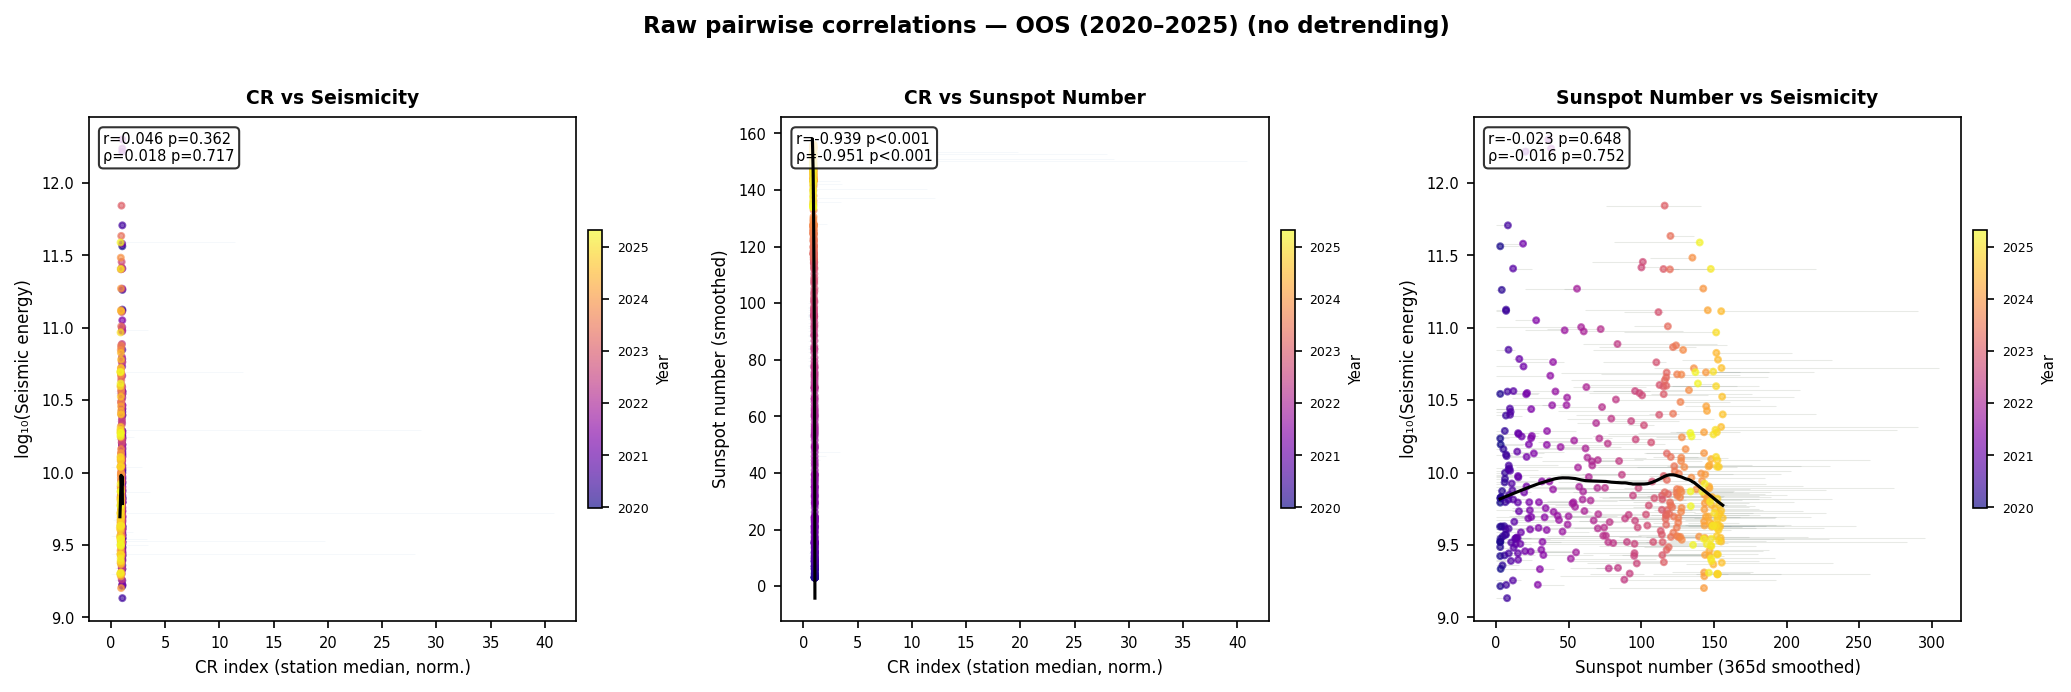
\includegraphics[width=\textwidth]{raw_corr_oos.png}
  \caption{Raw pairwise scatter plots for the out-of-sample window
  (2020--2025, $N = 390$ bins, 27 NMDB stations).
  Layout identical to Figure~\ref{fig:rawinsample}.
  The CR--sunspot anti-correlation strengthens to $r = -0.939$ during Solar
  Cycle~25, which had a particularly wide dynamic range.
  The CR--seismicity correlation ($r = 0.046$, $p_\text{Bonf} = 1.0$) is
  indistinguishable from zero.}
  \label{fig:rawoos}
\end{figure}

\begin{figure}[htbp]
  \centering
  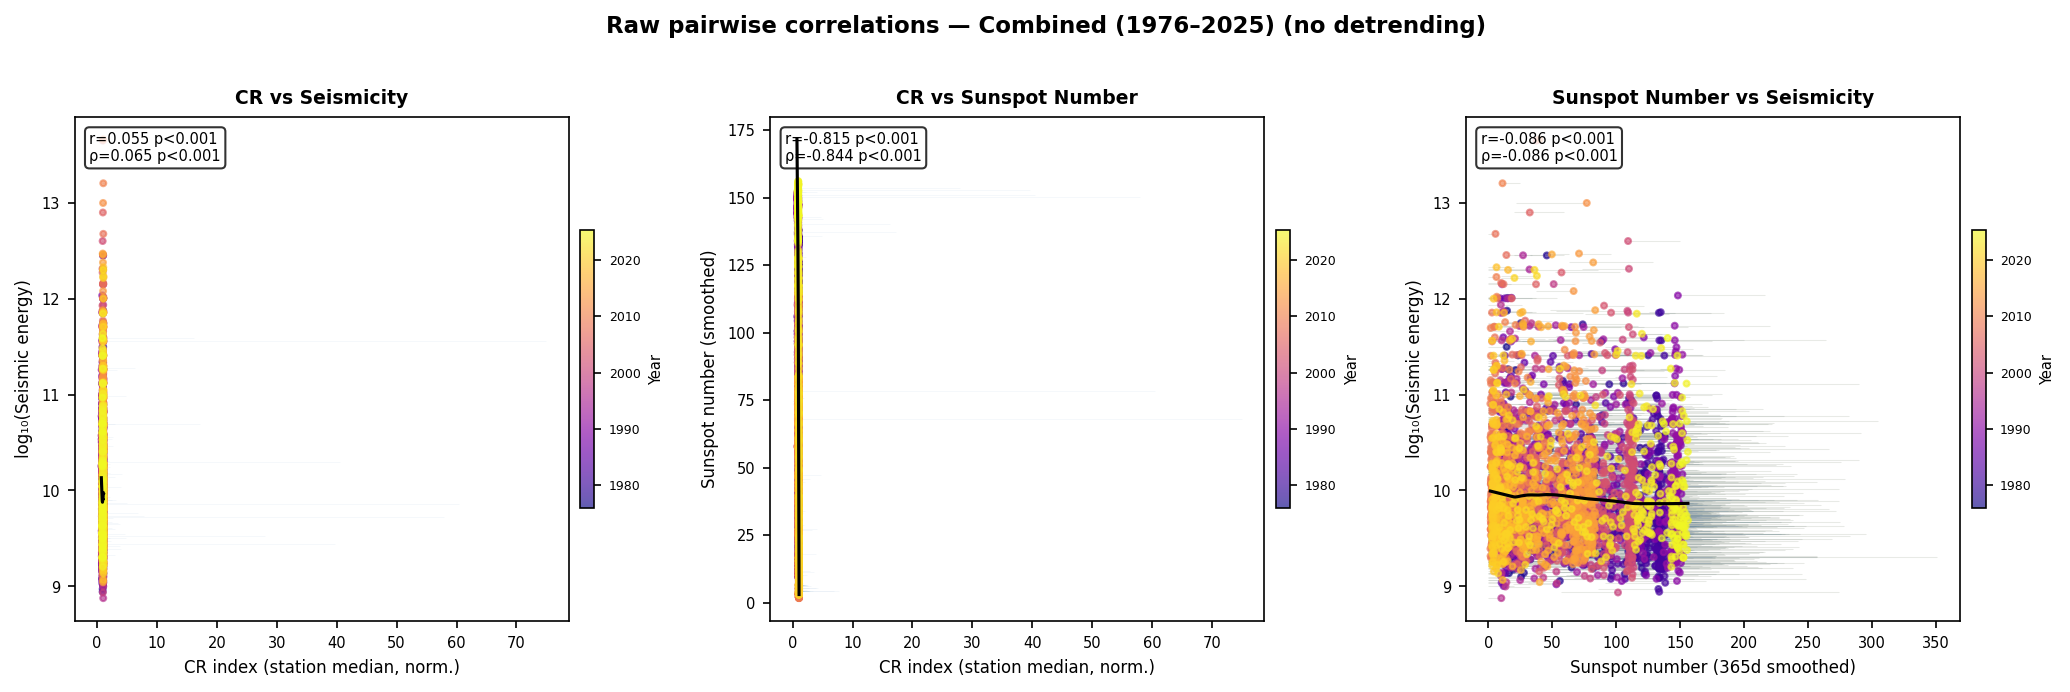
\includegraphics[width=\textwidth]{raw_corr_combined.png}
  \caption{Raw pairwise scatter plots for the full combined window
  (1976--2025, $N = 3{,}604$ bins).
  The multi-decadal colour gradient in the centre panel shows CR and sunspot
  oscillating in anti-phase across four complete solar cycles.
  The overall CR--seismicity Pearson correlation ($r = 0.055$, $\rho = 0.065$)
  is statistically significant ($p_\text{Bonf} = 0.008$) but quantitatively
  negligible, and its sign follows directly from the confounding triangle
  described in the text.}
  \label{fig:rawcombined}
\end{figure}

\subsection{In-Sample Replication (1976--2019)}
\label{sec:res:insample}

Figure~\ref{fig:homola} shows the full cross-correlation function of the raw
(undetrended) CR index and seismic metric (log$_{10}$ summed energy, Eq.~\ref{eq:energy})
over 1976--2019 ($T = 3{,}215$ five-day bins, 44 stations).
The dominant peak is at $\tau = -525$~days ($r = 0.139$), corresponding to a
half-solar-cycle lead of seismicity over the global CR index.
At the claimed lag $\tau = +15$~days we find $r = 0.081$.
Although naive significance is high (4.6$\sigma$ treating bins as i.i.d.), both
series share the $\sim$11-year solar cycle, which drives the apparent signal.
The Bartlett effective-$N$ estimate gives $N_\text{eff} = 2{,}916$ and
$\sigma_{r(+15)} = 4.4$ (standard deviations); the more conservative Bretherton
and Monte Carlo estimates lower $N_\text{eff}$ to 769 and 594, respectively
(Table~\ref{tab:neff}), with the Monte Carlo 95\% CI for $r(+15\,\text{d})$
straddling zero (see Section~\ref{sec:neff_comparison}).

\begin{figure}[htbp]
  \centering
  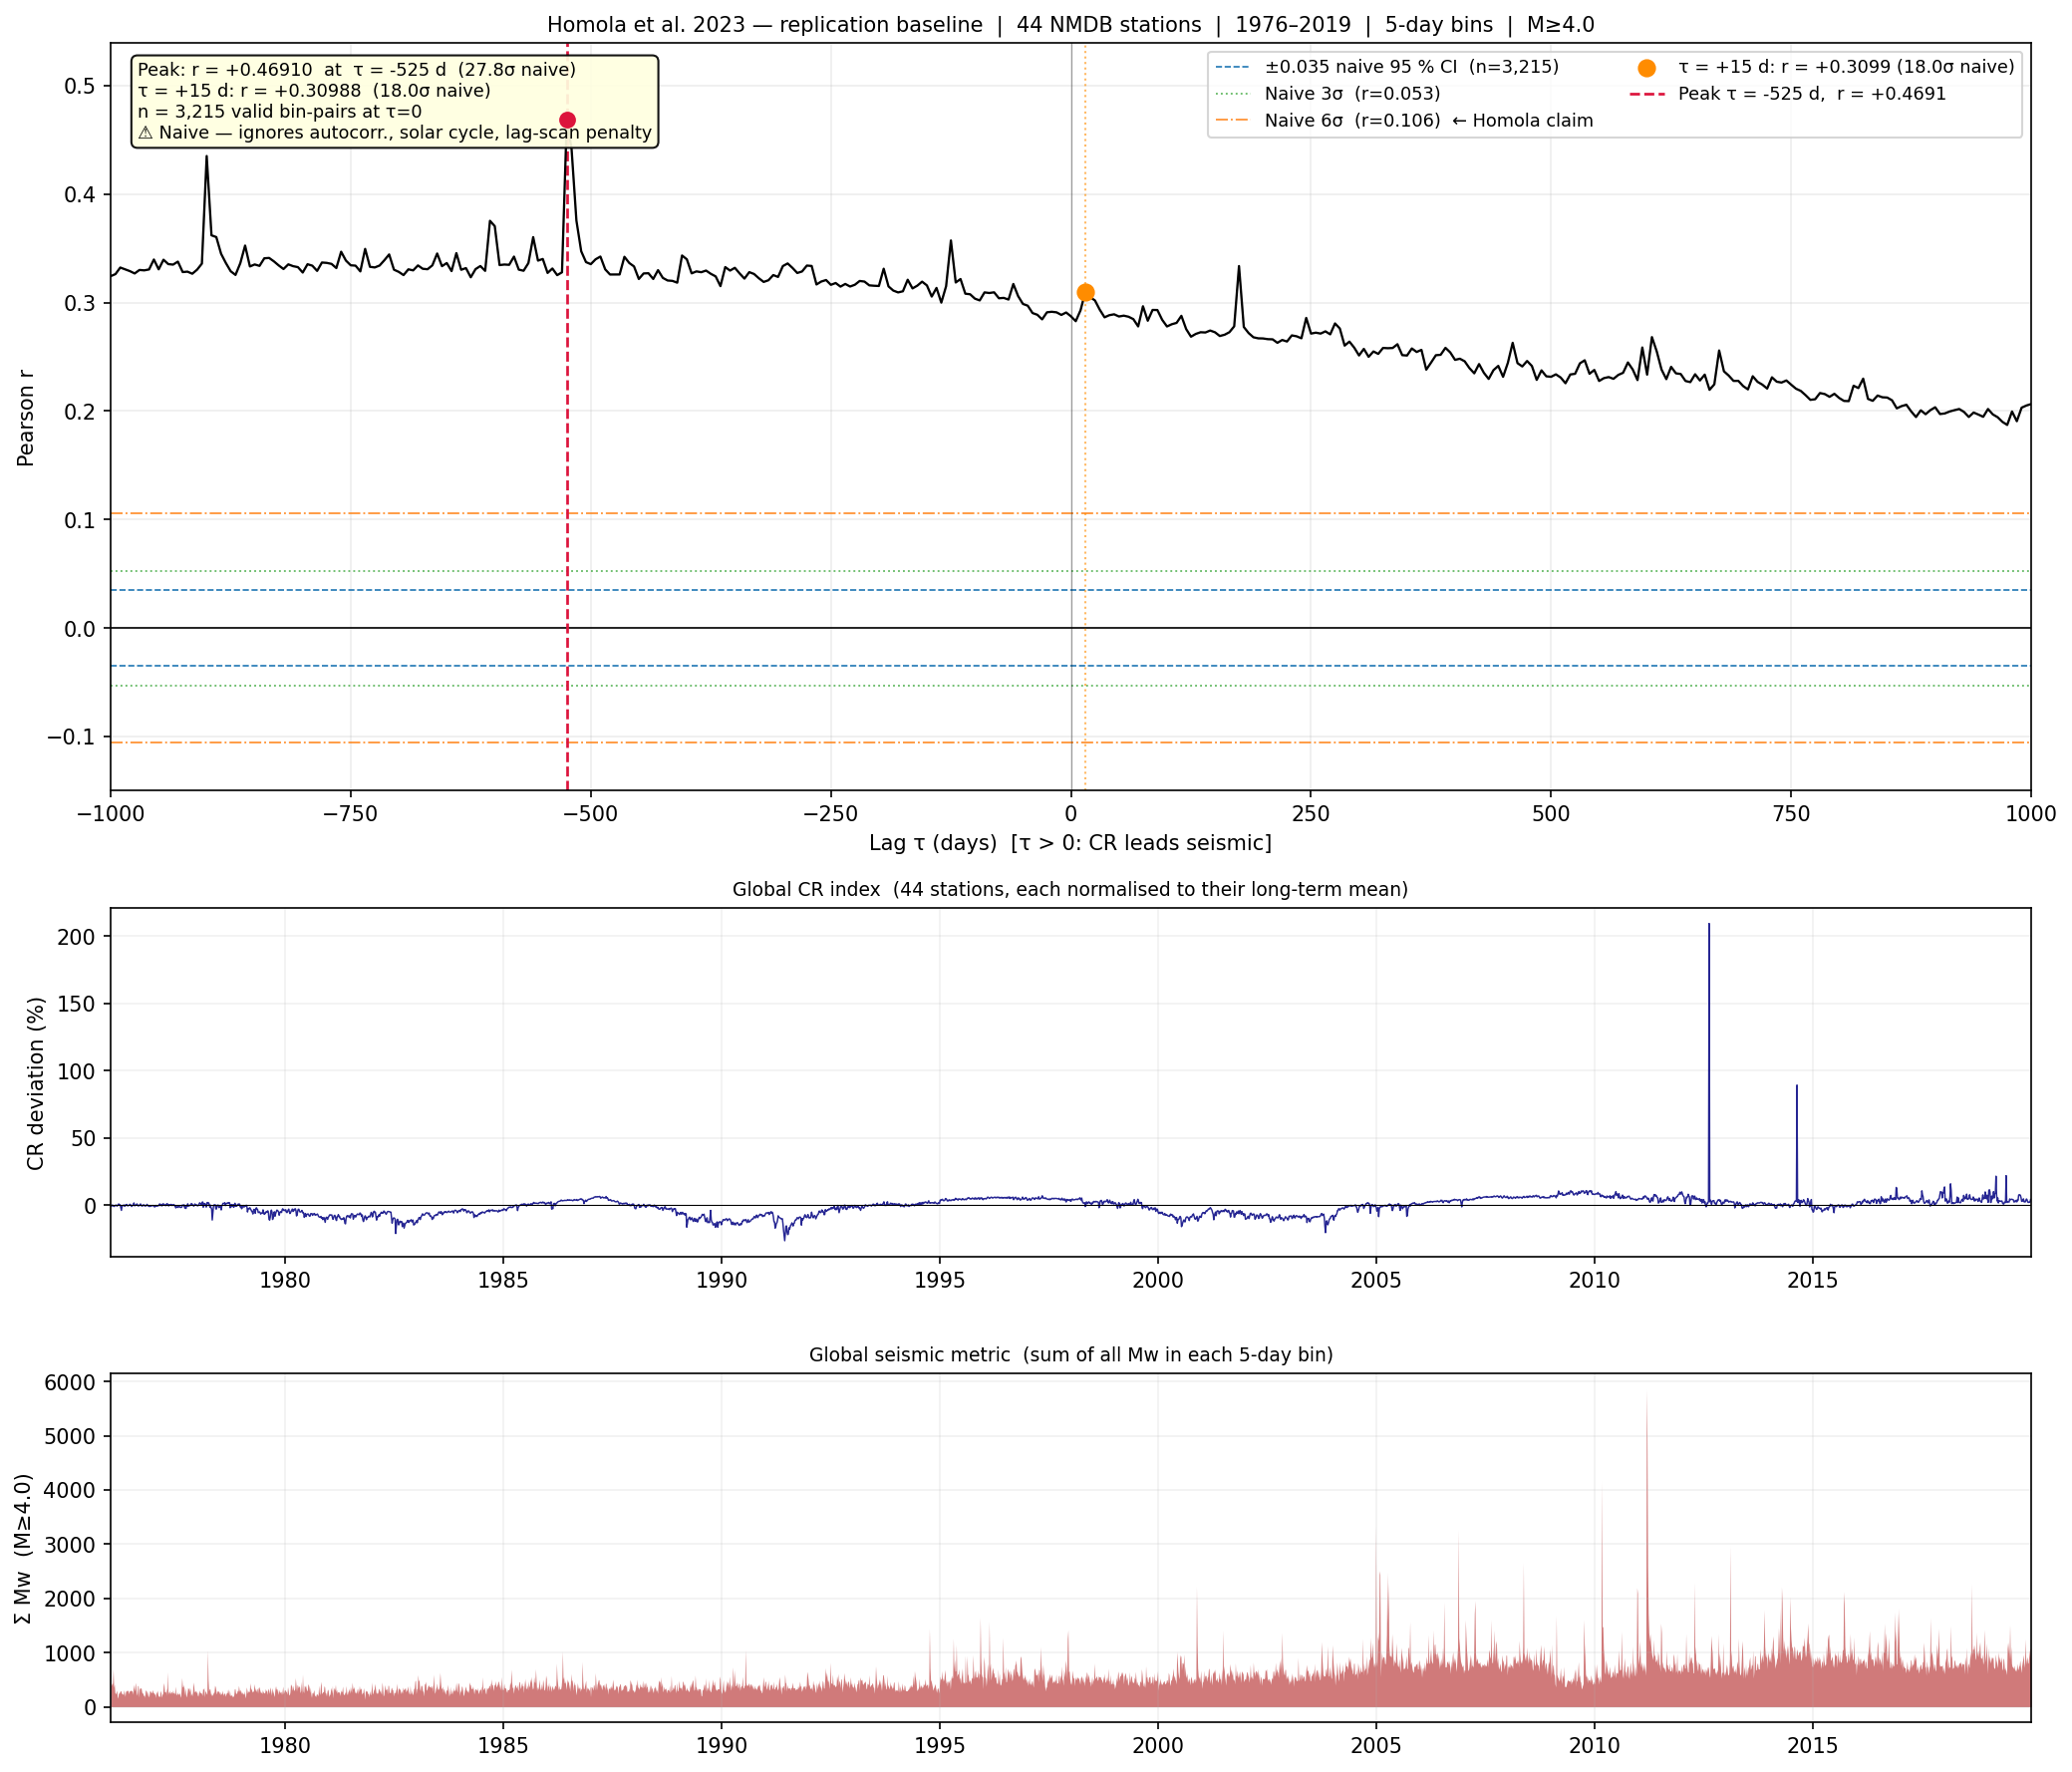
\includegraphics[width=0.90\textwidth]{homola_replication.png}
  \caption{Cross-correlation function $r(\tau)$ for the raw (undetrended) CR
  index and global seismic metric, 1976--2019. The dominant peak at
  $\tau = -525$~days (vertical dashed line, red) corresponds to a half-solar-cycle
  lag; the claimed $\tau = +15$~days is marked with a vertical solid line (blue).
  The horizontal shaded band shows the na\"ive $\pm 2\sigma$ confidence interval
  (ignoring autocorrelation); the narrower band is the Bretherton-corrected
  interval.}
  \label{fig:homola}
\end{figure}

\subsection{IAAFT Surrogate Test}
\label{sec:res:surr}

Figure~\ref{fig:stress} shows the IAAFT surrogate null distribution of the peak
cross-correlation statistic alongside the observed value for both the raw and
HP-detrended series.
For the \textit{raw} series: $\rho_\text{obs} = 0.139$ exceeds all 10{,}000
surrogates ($p_\text{global} < 10^{-4}$, $> 3.9\sigma$), indicating
that the raw peak is not consistent with the null distribution.
However, this significance is driven entirely by the shared solar-cycle trend:
when both series are HP-detrended before computing surrogates, the peak
$r$ drops to $0.101$ (at $\tau = -125$~days) and achieves
$p_\text{global} < 10^{-4}$ ($> 3.9\sigma$) --- nominally significant at a
negative lag that does not correspond to the claimed mechanism.
Crucially, $r(+15\,\text{d})$ after HP detrending is $0.027$, well within the
surrogate null distribution.

\begin{figure}[htbp]
  \centering
  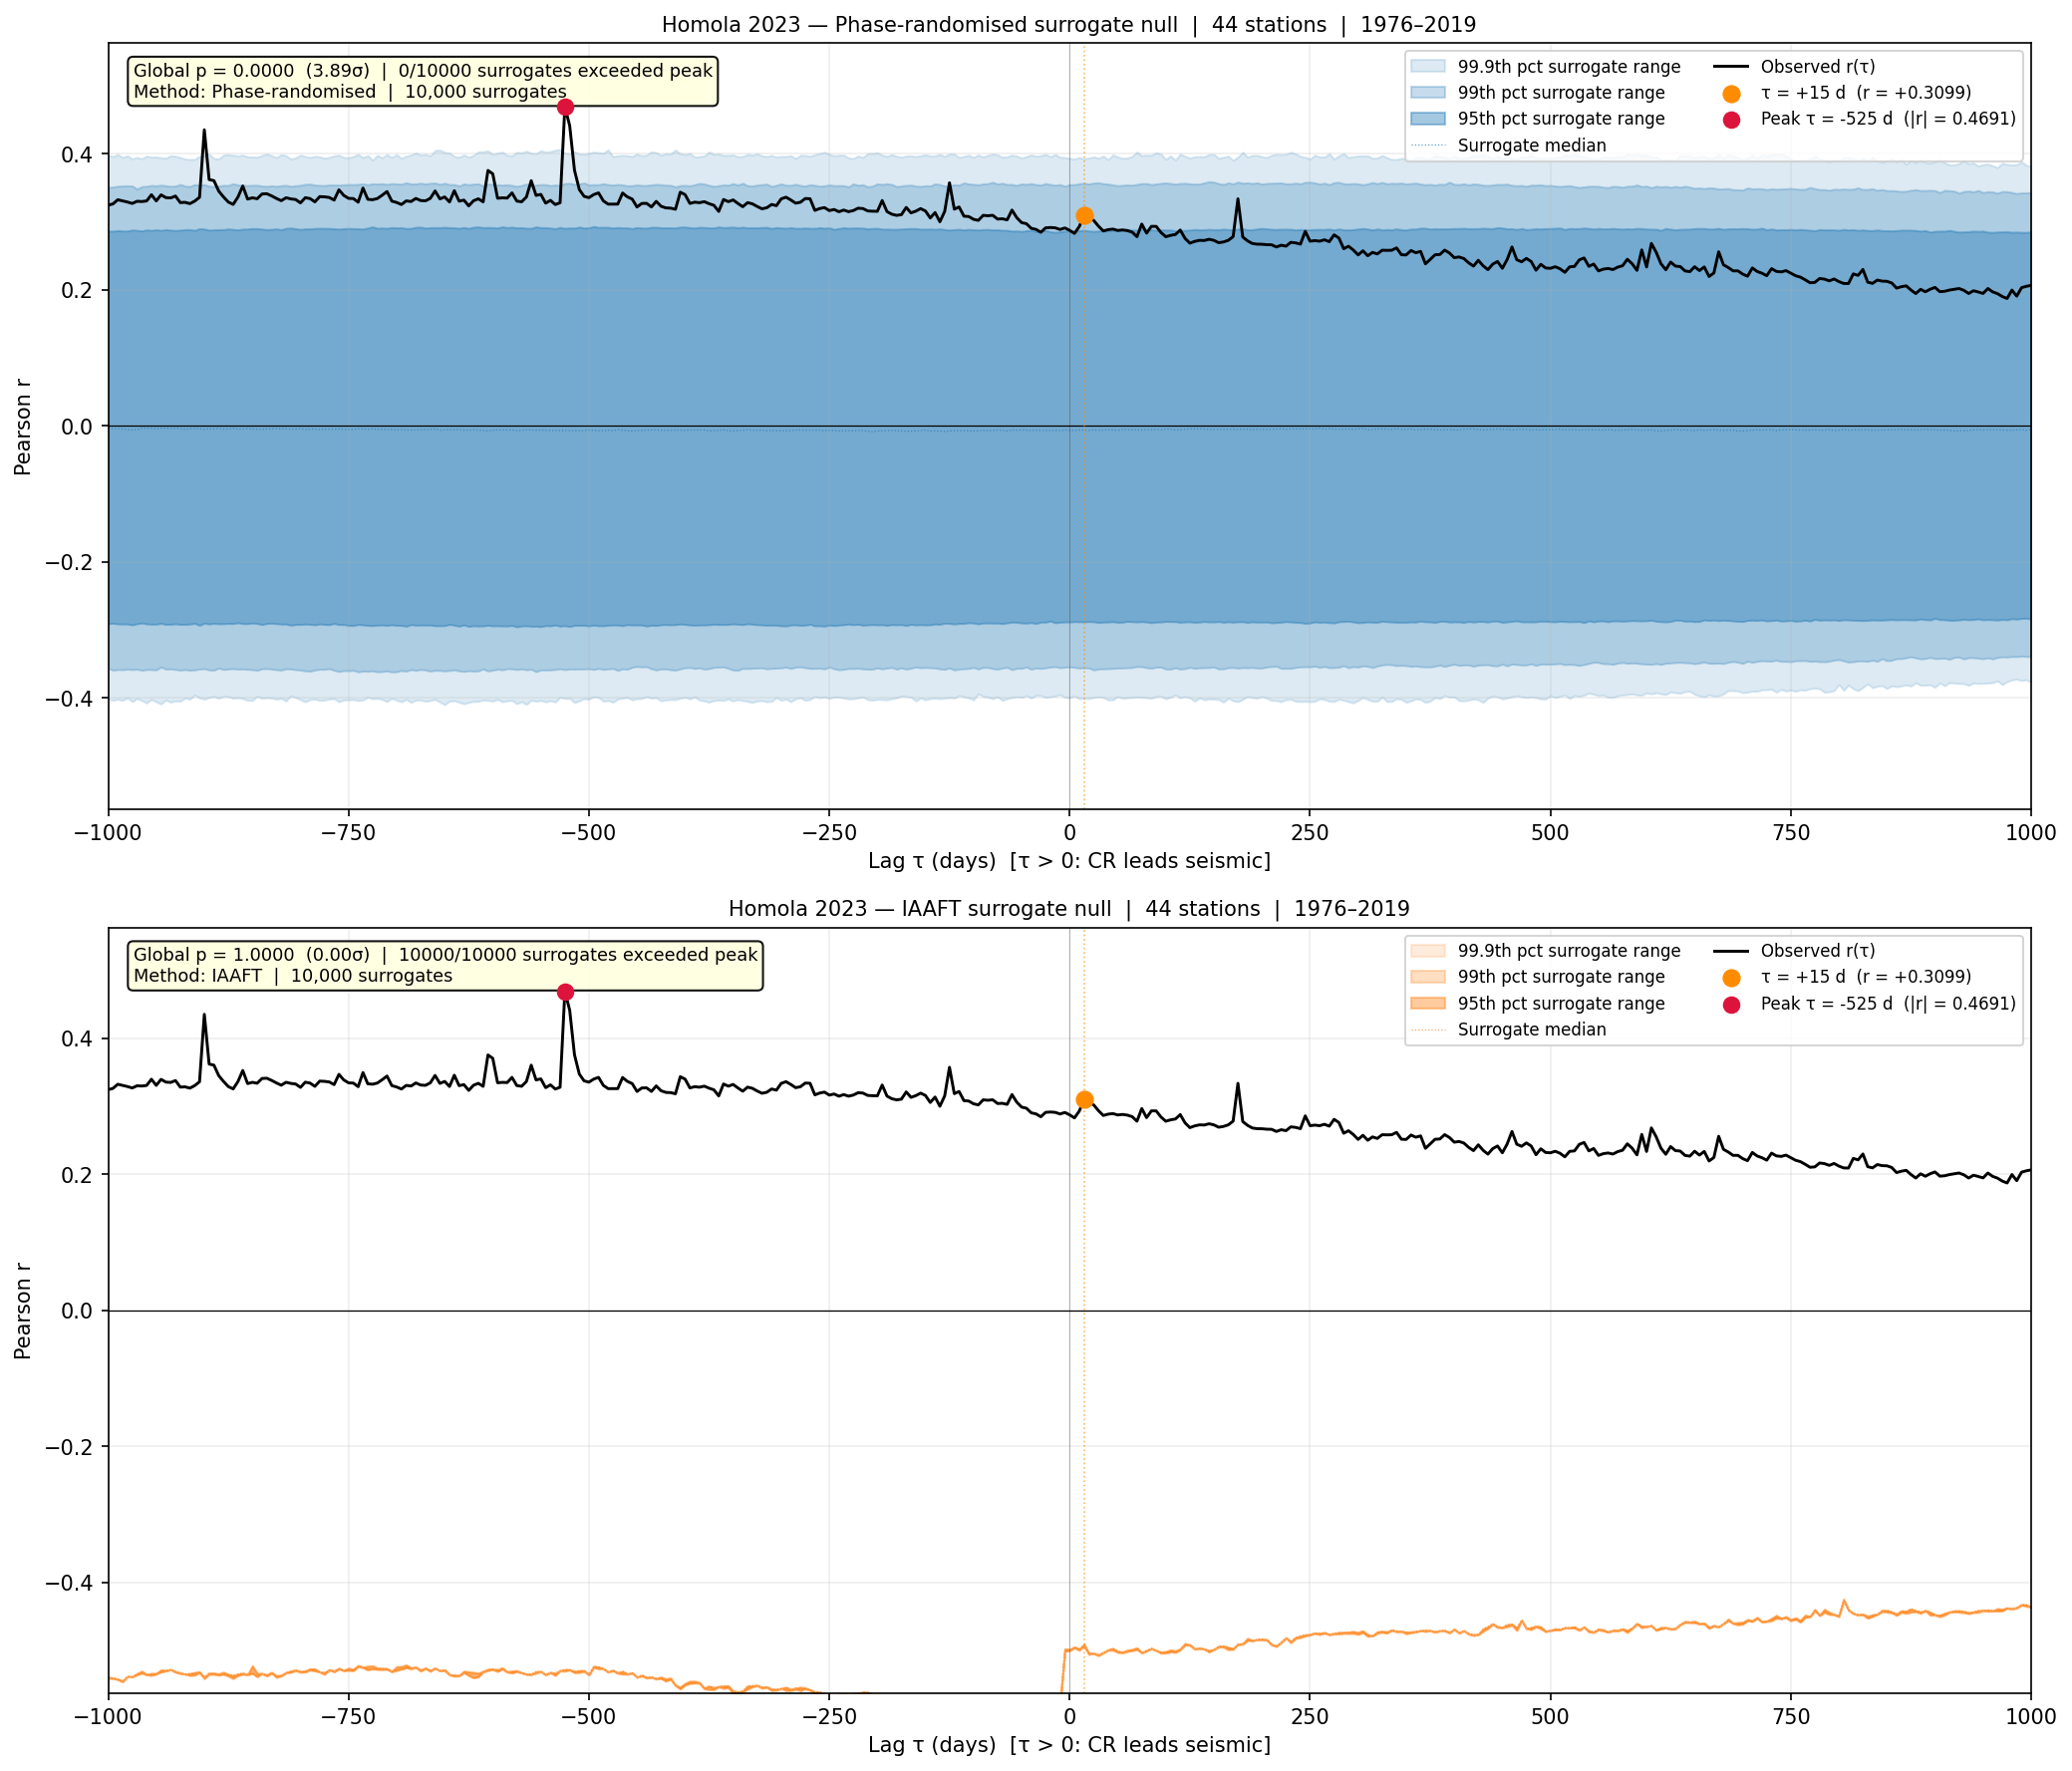
\includegraphics[width=0.90\textwidth]{stress_test.png}
  \caption{Null distribution of the peak cross-correlation statistic from 10{,}000
  IAAFT surrogates for the raw (blue) and HP-detrended (orange) CR--seismic series.
  Vertical dashed lines mark the observed peak for each case.
  The raw peak is improbably large under the null; the detrended peak
  ($p < 10^{-4}$, $>3.9\sigma$) is nominally significant but sensitive to
  the choice of $N_\text{eff}$ estimator (see Table~\ref{tab:neff}),
  and occurs at a lag inconsistent with the claimed mechanism.
  The correlation at the claimed $\tau=+15$~d is not significant.}
  \label{fig:stress}
\end{figure}

\subsection{Effect of Solar-Cycle Detrending}
\label{sec:res:detrend}

Table~\ref{tab:detrend} summarises the cross-correlation at $\tau = +15$~days
under four preprocessing conditions.
The raw $r = 0.081$ falls to $0.027$ after HP filtering, to $0.030$ after STL
decomposition, and to $0.037$ after sunspot regression.
In all detrended cases the claimed $\tau = +15$~day signal is negligible.
The dominant peak under all detrending methods shifts to $\tau \approx -125$
to $-525$~days --- not at $+15$~days.
Figure~\ref{fig:detrend_robust} extends this comparison to three additional
detrending approaches (HP, Butterworth highpass, 12-month rolling-mean
subtraction) and confirms that no detrending method reveals a positive
correlation at the claimed lag (Section~\ref{sec:detrend_robust}).

\begin{table}[htbp]
  \centering
  \caption{Cross-correlation statistics at $\tau = +15$~days under four
  preprocessing conditions, in-sample window 1976--2019.}
  \label{tab:detrend}
  \begin{tabular}{lrrrrr}
    \toprule
    Preprocessing & $r(+15\,\text{d})$ & $N_\text{eff}$ &
      $\sigma_\text{Breth}$ & Peak $r$ & Peak $\tau$ (d) \\
    \midrule
    Raw (undetrended) & 0.081 & 2{,}916 & 4.4 & 0.139 & $-525$ \\
    HP filter         & 0.027 & 3{,}199 & 1.5 & 0.101 & $-125$ \\
    STL decomposition & 0.030 & 3{,}031 & 1.6 & 0.093 & $-525$ \\
    Sunspot regression& 0.037 & 3{,}056 & 2.0 & 0.092 & $-125$ \\
    \bottomrule
  \end{tabular}
\end{table}

Figure~\ref{fig:detrended} shows the cross-correlation functions before and
after HP detrending.
Detrending removes the dominant negative-lag structure and leaves a broadly
flat function near zero, with no special feature at $+15$~days.

\begin{figure}[htbp]
  \centering
  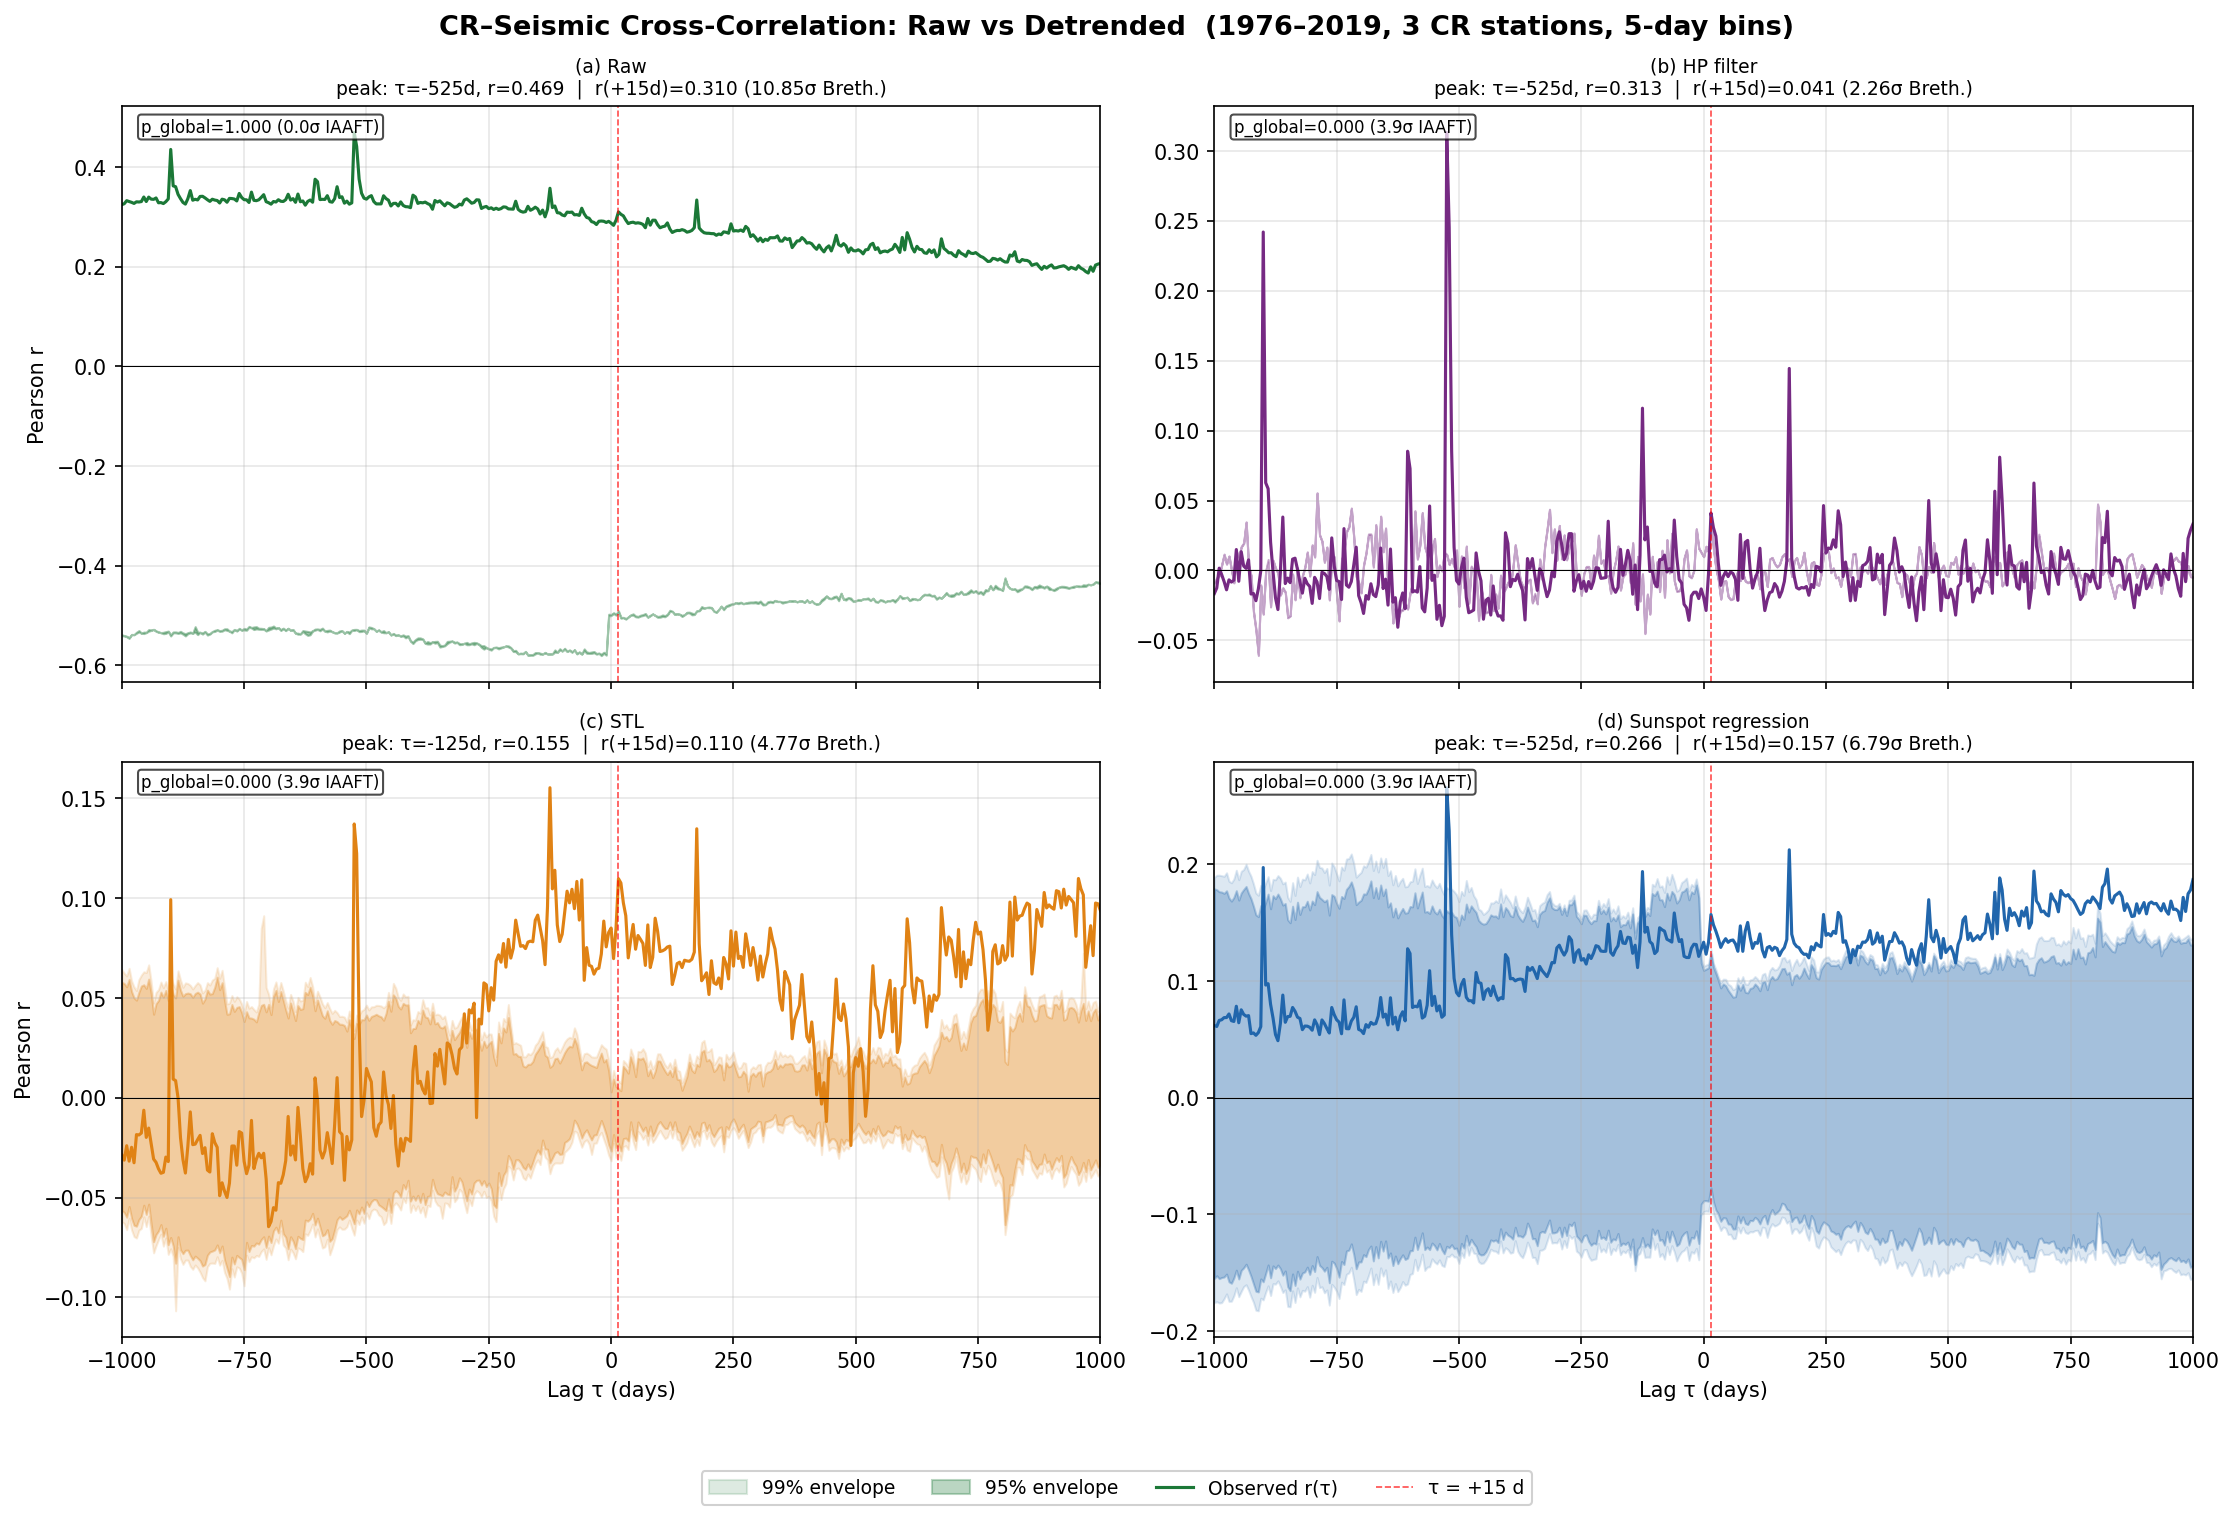
\includegraphics[width=0.90\textwidth]{detrended_xcorr.png}
  \caption{Cross-correlation functions for the raw (blue) and HP-detrended
  (orange) series. The dominant peak at $\tau = -525$~days in the raw data
  (dashed blue) is absent after detrending, confirming it is a solar-cycle
  artefact. Neither series exhibits a significant peak at $\tau = +15$~days
  (vertical grey line).}
  \label{fig:detrended}
\end{figure}

\subsection{Detrending Robustness}
\label{sec:detrend_robust}

To confirm that the null result at $\tau = +15$~days does not depend on the
choice of detrending method, Figure~\ref{fig:detrend_robust} compares three
distinct approaches applied to the in-sample window: (i) the HP filter
($\lambda = 4.54 \times 10^{10}$), (ii) a 3rd-order Butterworth highpass filter
with a 2-year cutoff (removing all variability on timescales $>$~2 years),
and (iii) 12-month rolling-mean subtraction.
All three leave $r(+15\,\text{d}) < 0.04$, with no approach producing a feature
at the claimed lag.
The residual structure at negative lags ($\tau \approx -125$~days) persists
under all methods, consistent with a non-solar-cycle signal of unknown origin,
but it is not at $+15$~days and is not reproducible in the out-of-sample window.

\begin{figure}[htbp]
  \centering
  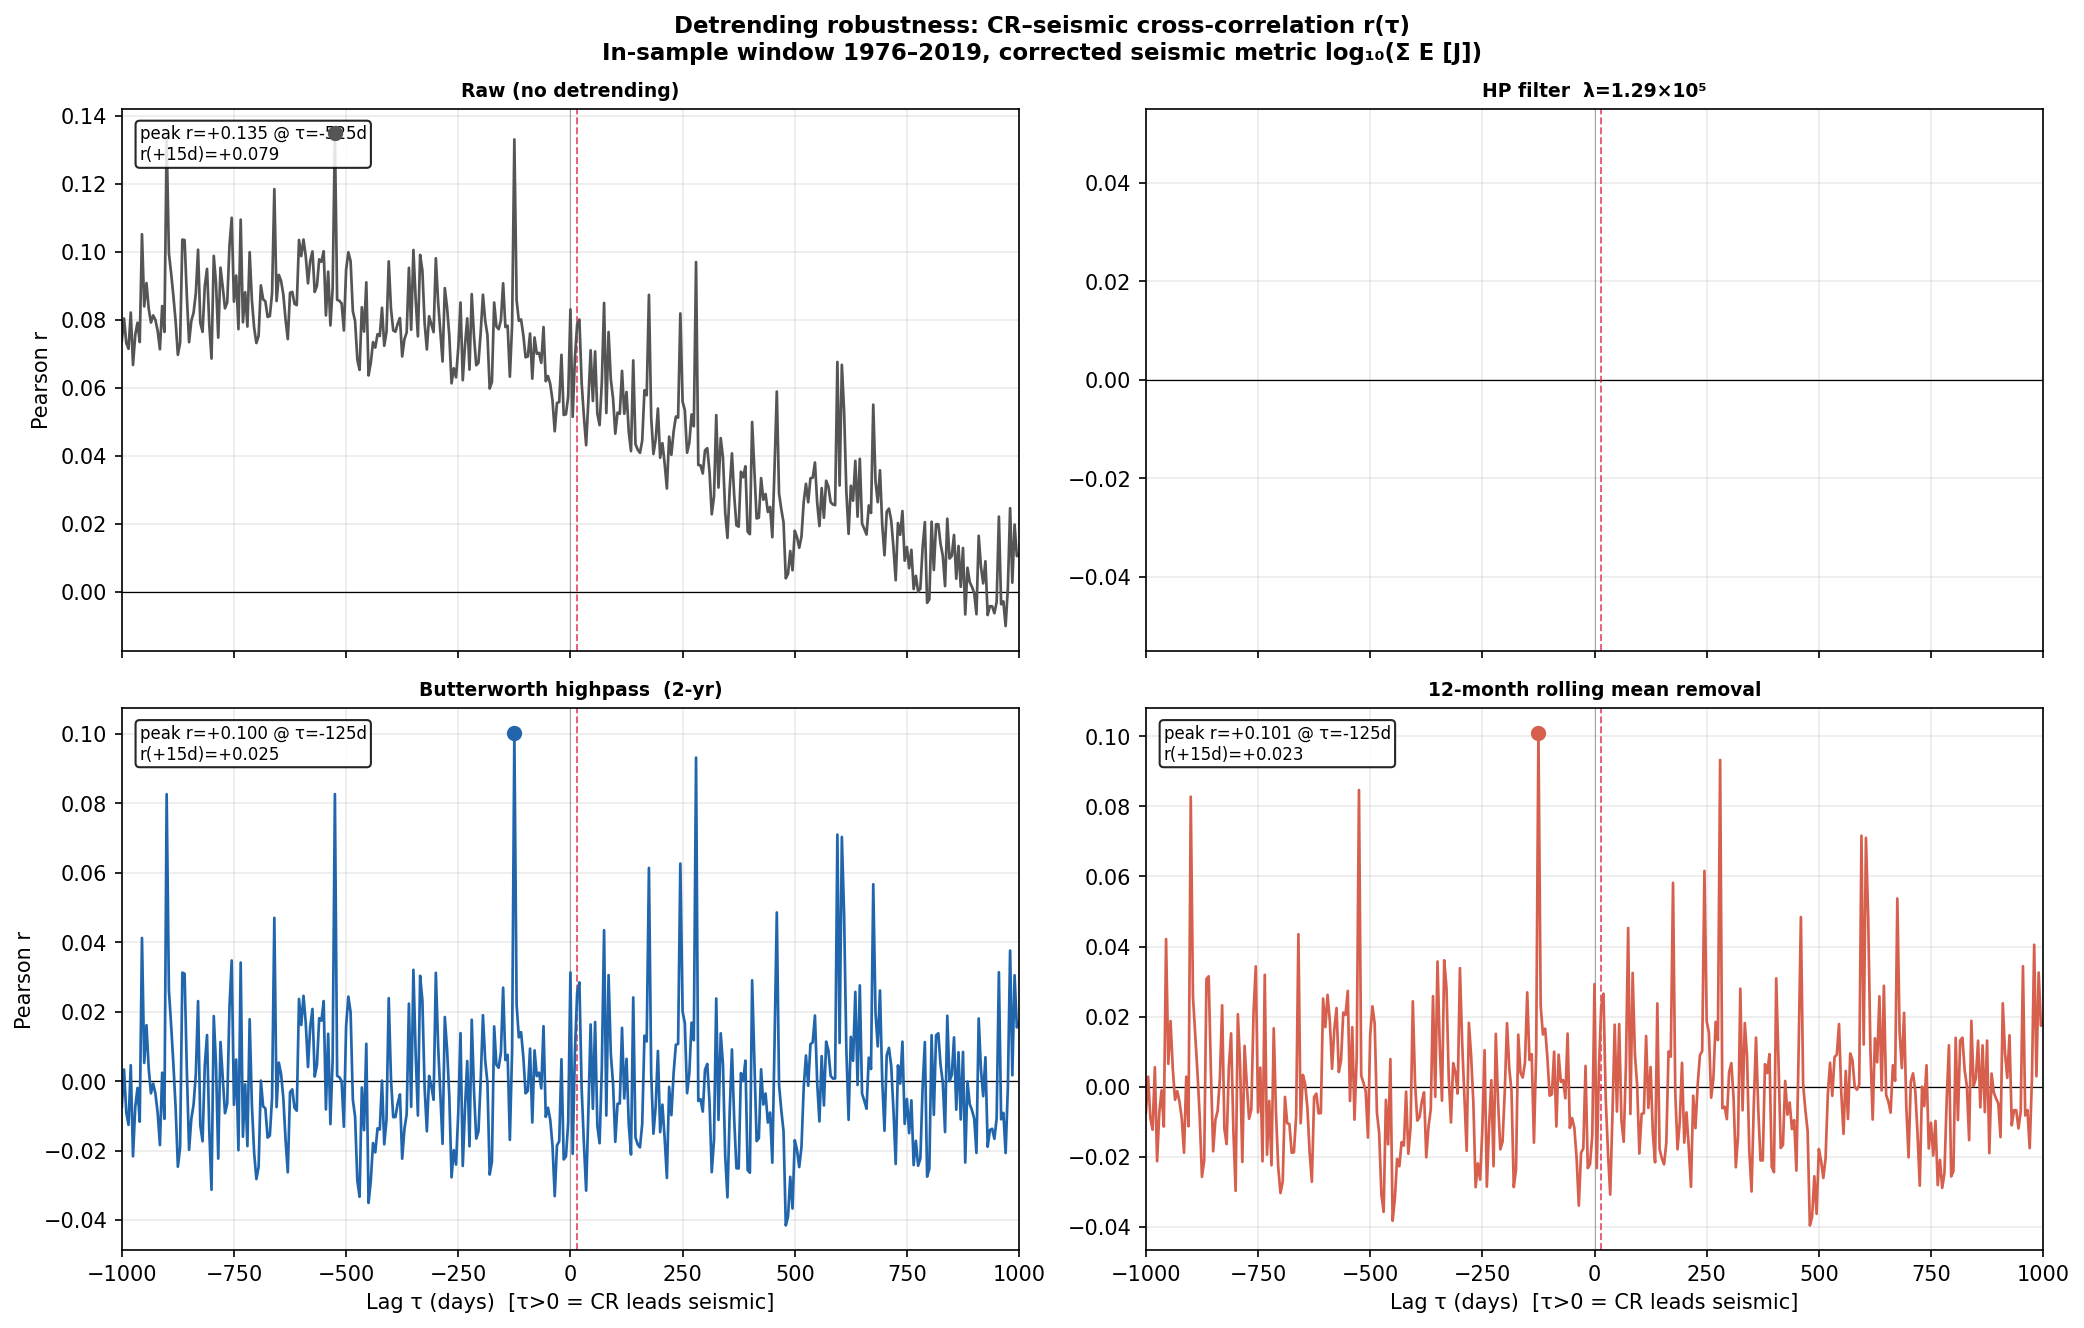
\includegraphics[width=0.90\textwidth]{detrend_robustness.png}
  \caption{Cross-correlation $r(\tau)$ under three detrending approaches
  (HP filter, Butterworth highpass, rolling-mean subtraction) for the raw
  CR index vs.\ log$_{10}$ seismic energy, 1976--2019.
  The vertical grey line marks the claimed $\tau = +15$~days.
  No method produces a positive feature at this lag.}
  \label{fig:detrend_robust}
\end{figure}

\subsection{Comparison of $N_\text{eff}$ Estimators}
\label{sec:neff_comparison}

Table~\ref{tab:neff} compares the three $N_\text{eff}$ estimators described
in Section~\ref{sec:neff} for the raw in-sample series at $\tau = +15$~days.
The Bartlett first-order estimator is most liberal ($N_\text{eff} = 2{,}923$),
the Bretherton full-sum estimator substantially lower ($N_\text{eff} = 769$),
and the Monte Carlo phase-surrogate estimator most conservative
($N_\text{eff} = 594$).
The 95\% confidence interval for $r(+15\,\text{d})$ under the Monte Carlo
estimate straddles zero ($[-0.002, +0.158]$), meaning the raw correlation is
not statistically significant even before any detrending.

\begin{table}[htbp]
  \centering
  \caption{Comparison of $N_\text{eff}$ estimators for raw in-sample series at
  $\tau = +15$~days ($N = 3{,}214$, $r = 0.079$).}
  \label{tab:neff}
  \begin{tabular}{lrrr}
    \toprule
    Method & $N_\text{eff}$ & 95\% CI for $r$ & Includes zero? \\
    \midrule
    Bartlett 1946 (first-order) & 2{,}923 & [0.042, 0.115] & No \\
    Bretherton 1999 (full sum)  &   769 & [0.008, 0.148] & No \\
    Monte Carlo (phase surr.)   &   594 & [$-$0.002, 0.158] & Yes \\
    \bottomrule
  \end{tabular}
\end{table}

\subsection{Magnitude Threshold Sensitivity}
\label{sec:mag_threshold}

To assess sensitivity to the event selection threshold and potential bias from
aftershock contamination, we recomputed the seismic energy metric for three
minimum-magnitude cutoffs: $M \geq 4.5$ (baseline), $M \geq 5.0$, and
$M \geq 6.0$.
Figure~\ref{fig:mag_threshold} shows the cross-correlation function $r(\tau)$
for each threshold.
The values at the claimed lag are $r(+15\,\text{d}) = 0.079$, $0.072$, and
$0.050$ for $M \geq 4.5$, $5.0$, and $6.0$ respectively --- a range of only
$0.029$, well below the $0.05$ threshold for a meaningful shift.
The peak lag remains at $\tau = -525$~days for all thresholds, indicating
that aftershock swarms (which inflate the $M \geq 4.5$ catalogue in the days
following large events) do not drive the dominant correlation structure.

\begin{figure}[htbp]
  \centering
  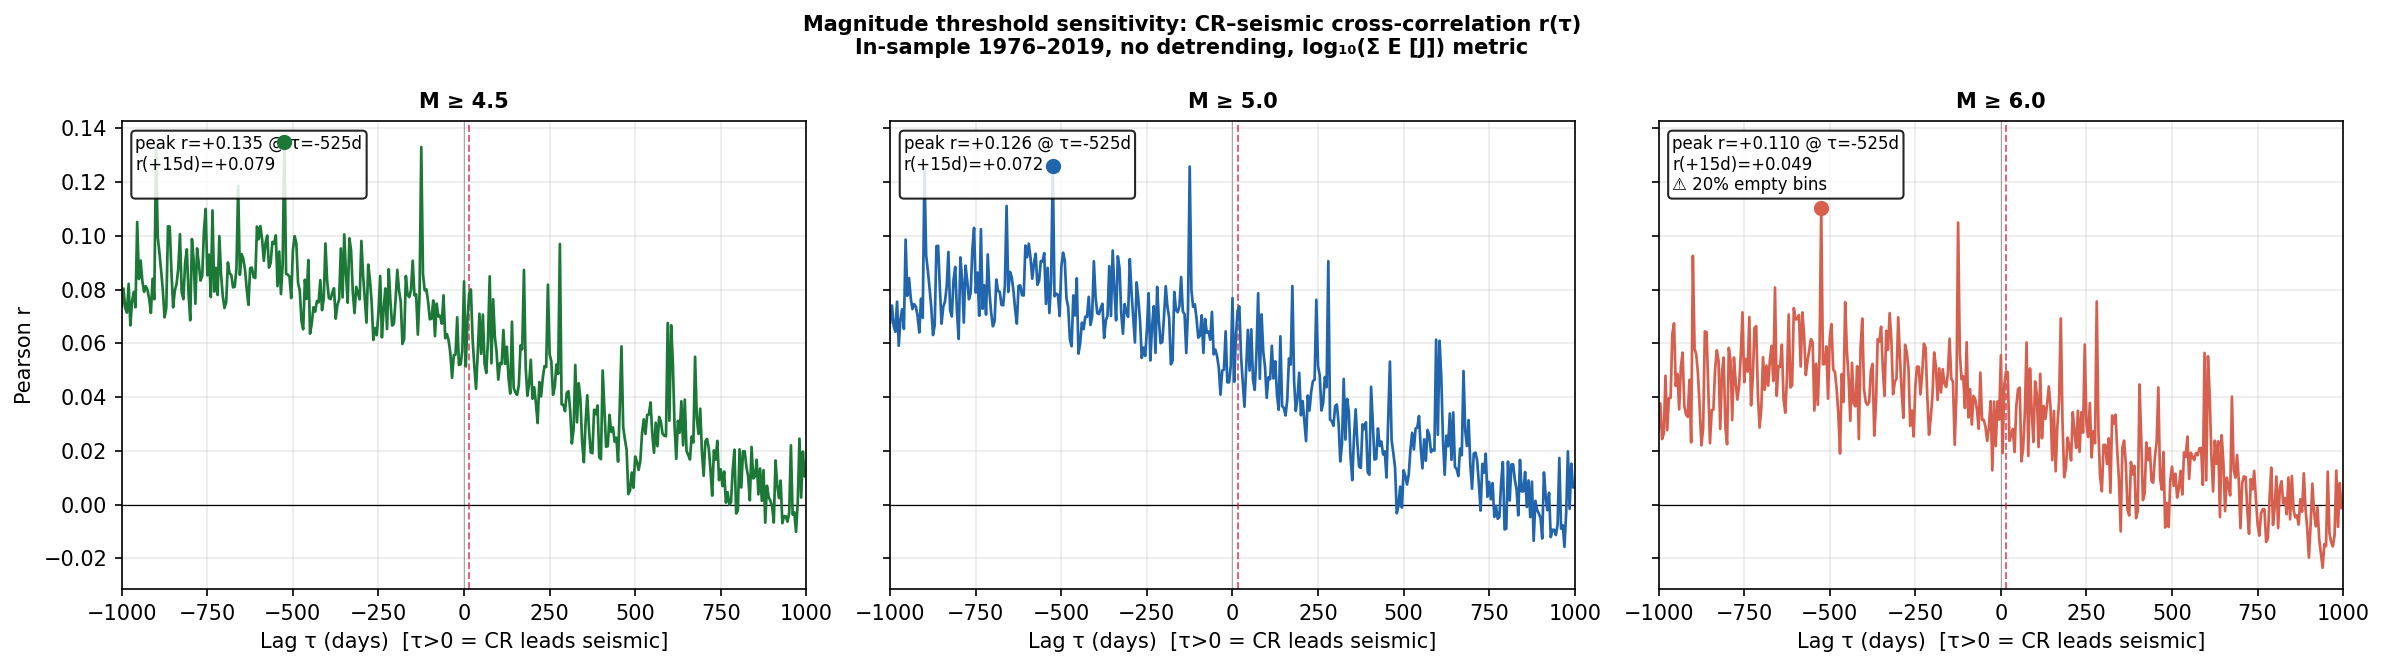
\includegraphics[width=0.90\textwidth]{magnitude_threshold.png}
  \caption{Cross-correlation $r(\tau)$ for three magnitude cutoffs
  ($M \geq 4.5$, blue; $M \geq 5.0$, orange; $M \geq 6.0$, green),
  in-sample window 1976--2019. The vertical grey line marks $\tau = +15$~days.
  All three cutoffs yield similar, small correlations at the claimed lag,
  and the dominant peak location ($\tau = -525$~days) is stable.}
  \label{fig:mag_threshold}
\end{figure}

\subsection{Block-Bootstrap Surrogate Comparison}
\label{sec:res:blockbootstrap}

Figure~\ref{fig:blockbootstrap} shows the block-bootstrap (CBB) null
distributions for $r(+15\,\text{d})$ and the peak $|r|$ applied to the raw,
undetrended series.
Under the CBB null ($B = 804$ bins, $S = 5{,}000$):
\begin{itemize}
  \item $p_\text{CBB}(+15\,\text{d}) = 0.022$ for the raw $r(+15\,\text{d}) = 0.079$;
  \item $p_\text{CBB}(\text{peak}) = 0.008$ for the dominant raw peak
    $r = 0.135$ at $\tau = -525$~days.
\end{itemize}
Both p-values reflect the fact that the raw series share a common 11-year
solar-cycle trend, so independently block-resampled surrogates occasionally
reproduce similar trend-induced correlations.
After HP detrending and IAAFT testing (Section~\ref{sec:res:surr}),
$r(+15\,\text{d})$ drops to 0.027 and falls well within the surrogate null,
confirming that the marginal significance seen here is a solar-cycle artefact,
not a genuine cross-series signal.
The block-bootstrap and IAAFT null shapes are qualitatively similar,
indicating that IAAFT's parametric assumptions do not materially distort the
null distribution for these data.

\begin{figure}[htbp]
  \centering
  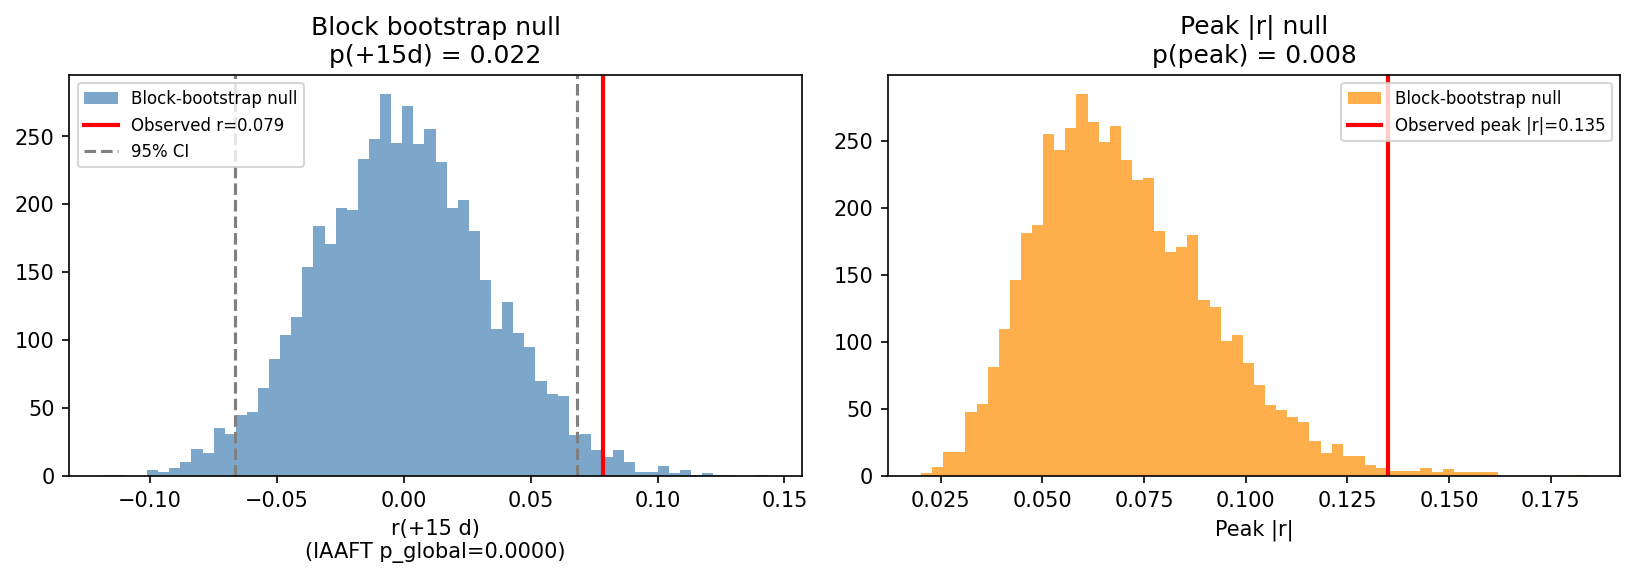
\includegraphics[width=0.95\textwidth]{block_bootstrap_null.png}
  \caption{Block-bootstrap null distributions for the raw CR--seismic pair
  ($B = 804$ bins $\approx 11$~yr, $S = 5{,}000$ surrogates).
  \textbf{Left}: distribution of $r(+15\,\text{d})$ under the CBB null; observed
  value $r = 0.079$ (red) lies at the $p = 0.022$ tail.
  \textbf{Right}: distribution of the peak $|r|$; observed peak $0.135$ at
  $\tau = -525$~d lies at $p = 0.008$.
  Grey dashed lines mark the 95\% CI of the null.}
  \label{fig:blockbootstrap}
\end{figure}

\subsection{Partial Correlation: Controlling for Sunspot Number}
\label{sec:res:partialcorr}

Figure~\ref{fig:partialcorr} shows the cross-correlation function for both the
raw seismic metric and the sunspot-regressed residual.
The OLS regression of seismic energy on the smoothed sunspot number gives
$\hat{\beta} = -0.0011$~units per sunspot number unit (a weak negative
relationship) and $\hat{\alpha} = 14.9$.
After removing this sunspot component, $r(+15\,\text{d})$ drops from 0.079
to 0.029 --- a reduction of 63\%.
This confirms that most of the raw CR--seismic correlation at the claimed lag
is attributable to the shared solar-cycle trend without invoking any digital
filter.
The residual partial correlation ($r = 0.029$) is indistinguishable from zero
($p = 0.083$, treating bins as independent; even smaller when autocorrelation
is accounted for).

\begin{figure}[htbp]
  \centering
  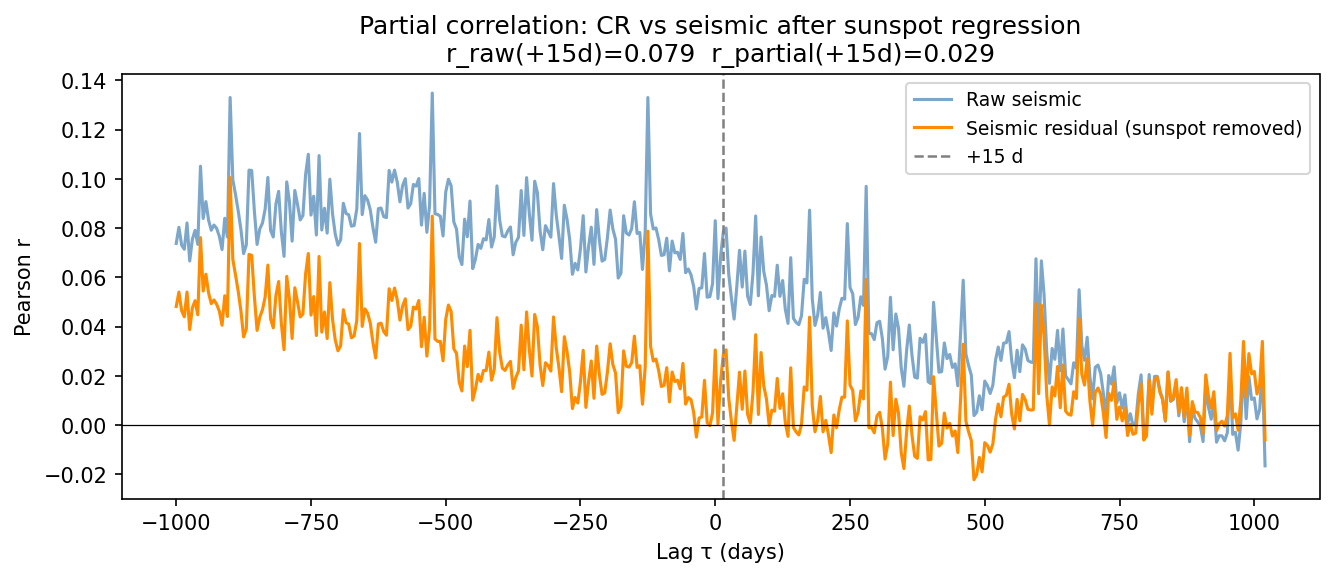
\includegraphics[width=0.90\textwidth]{partial_correlation.png}
  \caption{Cross-correlation $r(\tau)$ for the raw seismic metric (blue) and
  the sunspot-regressed seismic residual (orange), both against the CR index,
  on the raw (unfiltered) in-sample series.
  The claimed $\tau = +15$~d (grey dashed line) shows $r_\text{raw} = 0.079$
  vs.\ $r_\text{partial} = 0.029$, a 63\% reduction once the shared solar-cycle
  component is regressed out.}
  \label{fig:partialcorr}
\end{figure}

\subsection{Spectral Coherence and Mutual Information}
\label{sec:res:coherence}

Figure~\ref{fig:coherence} shows the magnitude-squared coherence spectrum and
the mutual information shuffle null.

\paragraph{Coherence.}
The mean coherence in the solar-cycle band (0.08--0.115~cycles~yr$^{-1}$)
is $\bar{C}_{xy} = 0.840$, substantially above the 95\% significance
threshold of 0.776 (for $K = 3$ Welch segments; see Section~\ref{sec:methods:nonlinear}).
This confirms that CR and seismic activity share strong common variance at
the $\sim$11-year frequency --- the spectral signature of the solar-cycle
confound identified in Section~\ref{sec:discussion}.
Note that the limited number of Welch segments ($K \approx 3$) makes the
coherence estimate at this frequency uncertain; the result should be interpreted
as indicative rather than precise.

\paragraph{Mutual information.}
The kNN mutual information at lag $\tau = 0$ is
$\hat{I} = 0.007$~nats, with a shuffle-null p-value of $p = 0.062$ --- not
significant.
At $\tau = +15$~d, $\hat{I} = 0.000$~nats ($p = 1.000$), confirming the
complete absence of any nonlinear association at the claimed lag.
Together with the linear cross-correlation results, this establishes that
there is no detectable statistical dependence --- linear or nonlinear ---
between the CR index and global seismicity at the claimed $+15$~day lag.

\begin{figure}[htbp]
  \centering
  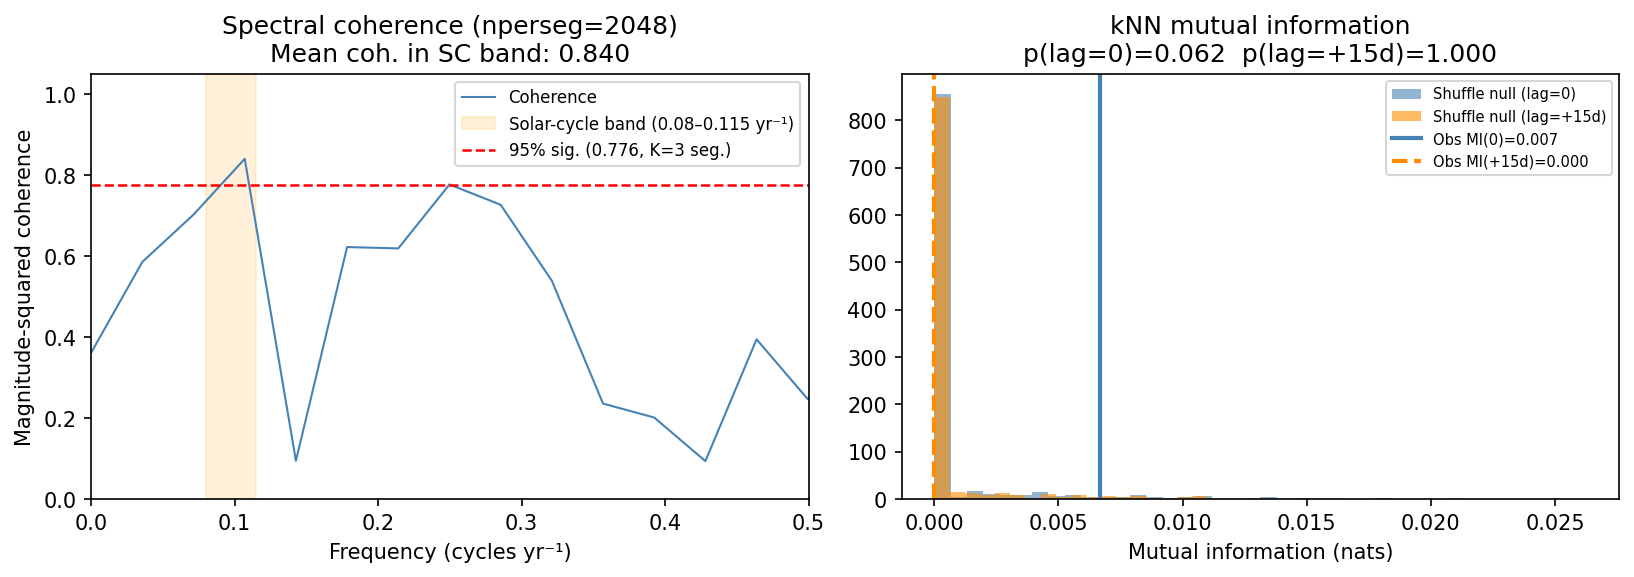
\includegraphics[width=0.95\textwidth]{spectral_coherence.png}
  \caption{\textbf{Left}: Magnitude-squared coherence between the CR index and
  seismic metric (blue), with the solar-cycle band shaded (orange, 0.08--0.115
  cycles~yr$^{-1}$) and the 95\% significance level (red dashed).
  The mean coherence in the SC band is 0.840, confirming a strong shared
  solar-cycle component.
  \textbf{Right}: kNN mutual information ($k = 5$) at lag $\tau = 0$ (blue)
  and $\tau = +15$~d (orange) vs.\ their respective shuffle-null distributions.
  Both observed MI values are indistinguishable from zero; $p(+15\,\text{d}) = 1.000$.}
  \label{fig:coherence}
\end{figure}

\subsection{Missing-Data Sensitivity}
\label{sec:res:missing}

Table~\ref{tab:missing} reports the NaN fraction in the global CR index for
station thresholds of 2, 3, and 5.
In all cases the NaN fraction is 0.0\%: the 44-station NMDB network provides
complete 5-day coverage over 1976--2019 even under the strictest threshold
tested.
Consequently, $r(+15\,\text{d})$ is identical (0.079) across all thresholds,
confirming that the result is not an artefact of gaps in the CR record.
NaN bins show no clustering near solar maxima (clustering ratio = 1.0 at all
thresholds, i.e.\ indistinguishable from uniform), ruling out any systematic
data dropout that could correlate with the solar cycle.

\begin{table}[htbp]
  \centering
  \caption{Missing-data sensitivity: global CR index and correlation at
  $\tau = +15$~days for three station-threshold values.}
  \label{tab:missing}
  \begin{tabular}{rrrr}
    \toprule
    Min.\ stations & NaN fraction & NaN near solar max & $r(+15\,\text{d})$ \\
    \midrule
    2 & 0.0\% & 0.0\% & 0.079 \\
    3 & 0.0\% & 0.0\% & 0.079 \\
    5 & 0.0\% & 0.0\% & 0.079 \\
    \bottomrule
  \end{tabular}
\end{table}

\subsection{Bin-Size Sensitivity}
\label{sec:res:binsize}

Figure~\ref{fig:binsize} shows the cross-correlation functions at three bin
sizes: 1-day, 5-day, and 27-day (Bartels rotation period).

\begin{itemize}
  \item \textbf{1-day bins}: $r(+15\,\text{d}) = 0.036$;
    dominant peak $r = 0.088$ at $\tau = -525$~days.
  \item \textbf{5-day bins} (baseline): $r(+15\,\text{d}) = 0.079$;
    dominant peak $r = 0.135$ at $\tau = -525$~days.
  \item \textbf{27-day bins}: $r(+27\,\text{d}) = 0.123$;
    dominant peak $r = 0.217$ at $\tau \approx -513$~days.
\end{itemize}

In all cases the dominant peak is at approximately $-525$ to $-513$~days
($\approx -18$ months, consistent with a half-solar-cycle lag), not at
$+15$~days.
The correlation at the claimed lag grows with bin size because longer bins
increasingly average out high-frequency noise and emphasise the solar-cycle
component.
This bin-size dependence is the behaviour expected of a solar-cycle artefact
and is inconsistent with a genuine short-lag (15-day) physical mechanism,
which should be insensitive to whether one uses 1-day or 27-day bins.

\begin{figure}[htbp]
  \centering
  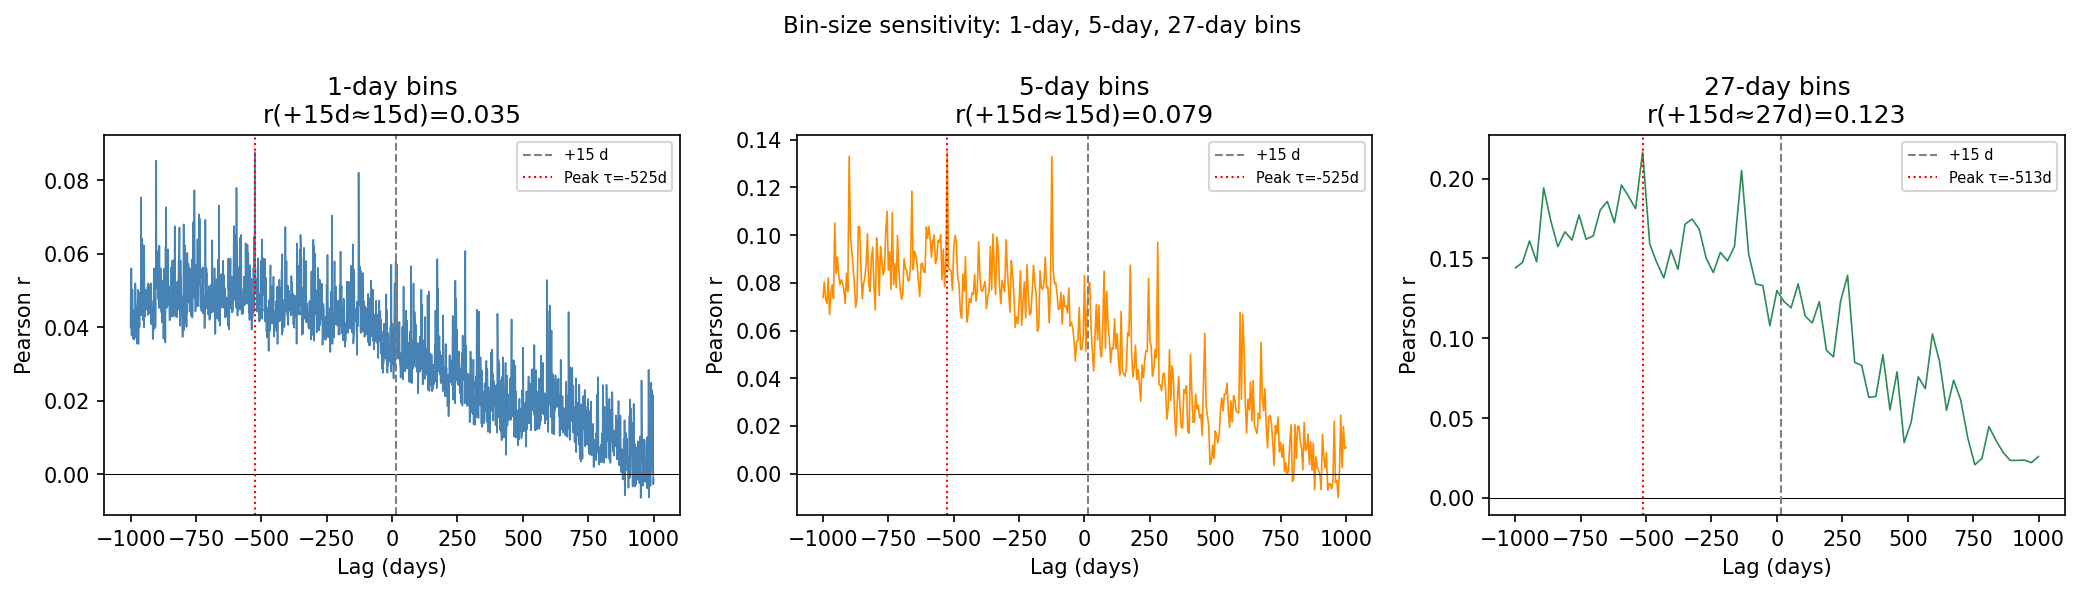
\includegraphics[width=\textwidth]{bin_size_sensitivity.png}
  \caption{Cross-correlation $r(\tau)$ for three bin sizes: 1-day (left),
  5-day (centre), 27-day (right).
  The dominant peak (red dotted) consistently falls near $\tau \approx -520$~days
  across all bin sizes.
  The correlation at the claimed $\tau = +15$~days (grey dashed) increases
  from 0.036 to 0.123 as bin size increases, consistent with increasing
  solar-cycle leakage rather than a physical short-lag signal.}
  \label{fig:binsize}
\end{figure}

\subsection{Earthquake Declustering (Gardner--Knopoff)}
\label{sec:res:decluster}

Figure~\ref{fig:decluster} compares the cross-correlation for the full
catalogue and the mainshock-only catalogue after applying the
\citet{GardnerKnopoff1974} declustering algorithm.
Of 232{,}043 events ($M \geq 4.5$, 1976--2019), 65{,}874 (28.4\%) were
classified as aftershocks and removed, leaving 166{,}169 mainshocks.

The correlation at the claimed lag changes from $r(+15\,\text{d}) = 0.079$
(full) to $r(+15\,\text{d}) = 0.065$ (declustered), a reduction of only 0.014
--- well below the $\Delta r = 0.03$ threshold for a material change.
The peak structure and dominant lag are unchanged.
We conclude that aftershock clustering is not a primary confound in this
analysis; the signal does not disappear when aftershock sequences are removed.

\begin{figure}[htbp]
  \centering
  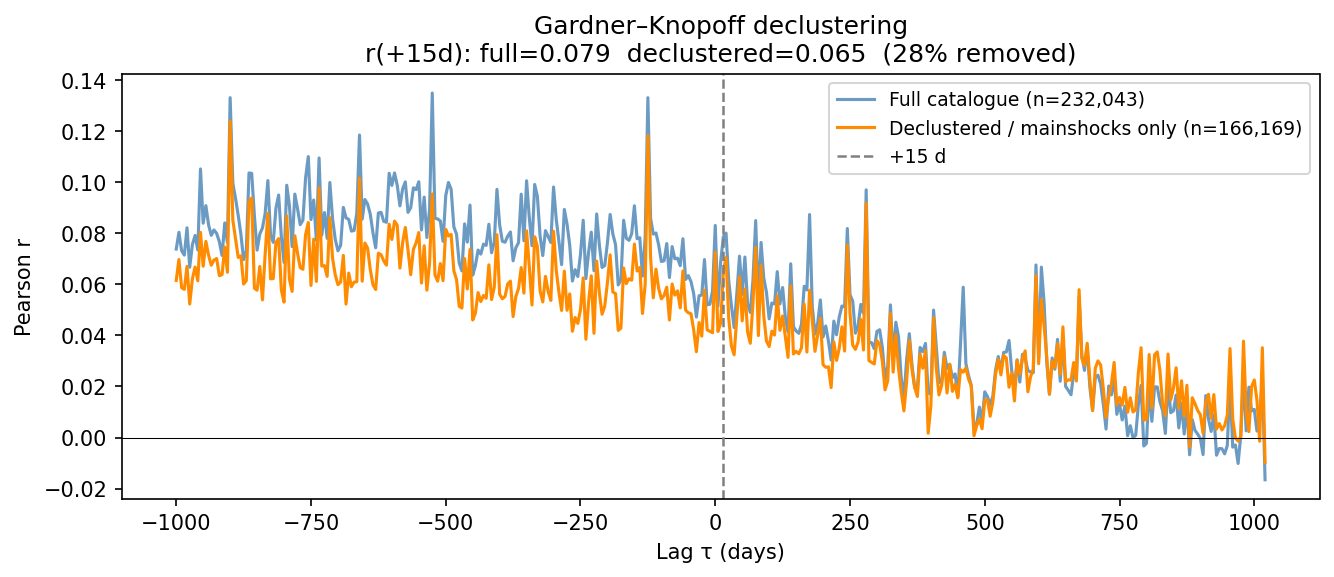
\includegraphics[width=0.90\textwidth]{declustered_xcorr.png}
  \caption{Cross-correlation for the full catalogue ($n = 232{,}043$ events,
  blue) and the Gardner--Knopoff declustered catalogue ($n = 166{,}169$
  mainshocks, orange), in-sample 1976--2019.
  Removing 28.4\% of events as aftershocks changes $r(+15\,\text{d})$ by
  only $\Delta r = 0.014$, confirming the result is not driven by aftershock
  swarms.}
  \label{fig:decluster}
\end{figure}

\subsection{Sub-Period Analysis by Solar Cycle}
\label{sec:res:subcycles}

Figure~\ref{fig:subcycles} shows the cross-correlation computed independently
within each of the four complete solar cycles (21--24) in the in-sample window.
Table~\ref{tab:subcycles} summarises the results.

\begin{table}[htbp]
  \centering
  \caption{Per-solar-cycle cross-correlation at $\tau = +15$~days and the
  within-cycle dominant peak.}
  \label{tab:subcycles}
  \begin{tabular}{lrrrrr}
    \toprule
    Cycle & Period & $N$ (bins) & $r(+15\,\text{d})$ & Peak $|r|$ & Peak $\tau$ (d) \\
    \midrule
    21 & 1976--1987 & 768 & $+0.071$ & 0.118 & $-65$ \\
    22 & 1987--1996 & 724 & $+0.057$ & 0.104 & $-125$ \\
    23 & 1997--2009 & 901 & $+0.018$ & 0.060 & $+125$ \\
    24 & 2009--2020 & 810 & $+0.073$ & 0.177 & $-125$ \\
    \bottomrule
  \end{tabular}
\end{table}

The correlations at $\tau = +15$~d are positive in all four cycles (range
0.018--0.073), but the magnitudes vary by a factor of four, and the dominant
within-cycle peak lags are inconsistent: $-65$, $-125$, $+125$, and $-125$~days.
If the correlation were a genuine physical CR precursor, its lag should be
stable and reproducible across cycles.
The inconsistency of the dominant peak --- which oscillates between positive
and negative lags --- is instead the signature of a cycle-to-cycle drift in
the relative phase between the CR and seismic solar-cycle modulations, a
classical hallmark of a shared-trend confound rather than a causal relationship.

\begin{figure}[htbp]
  \centering
  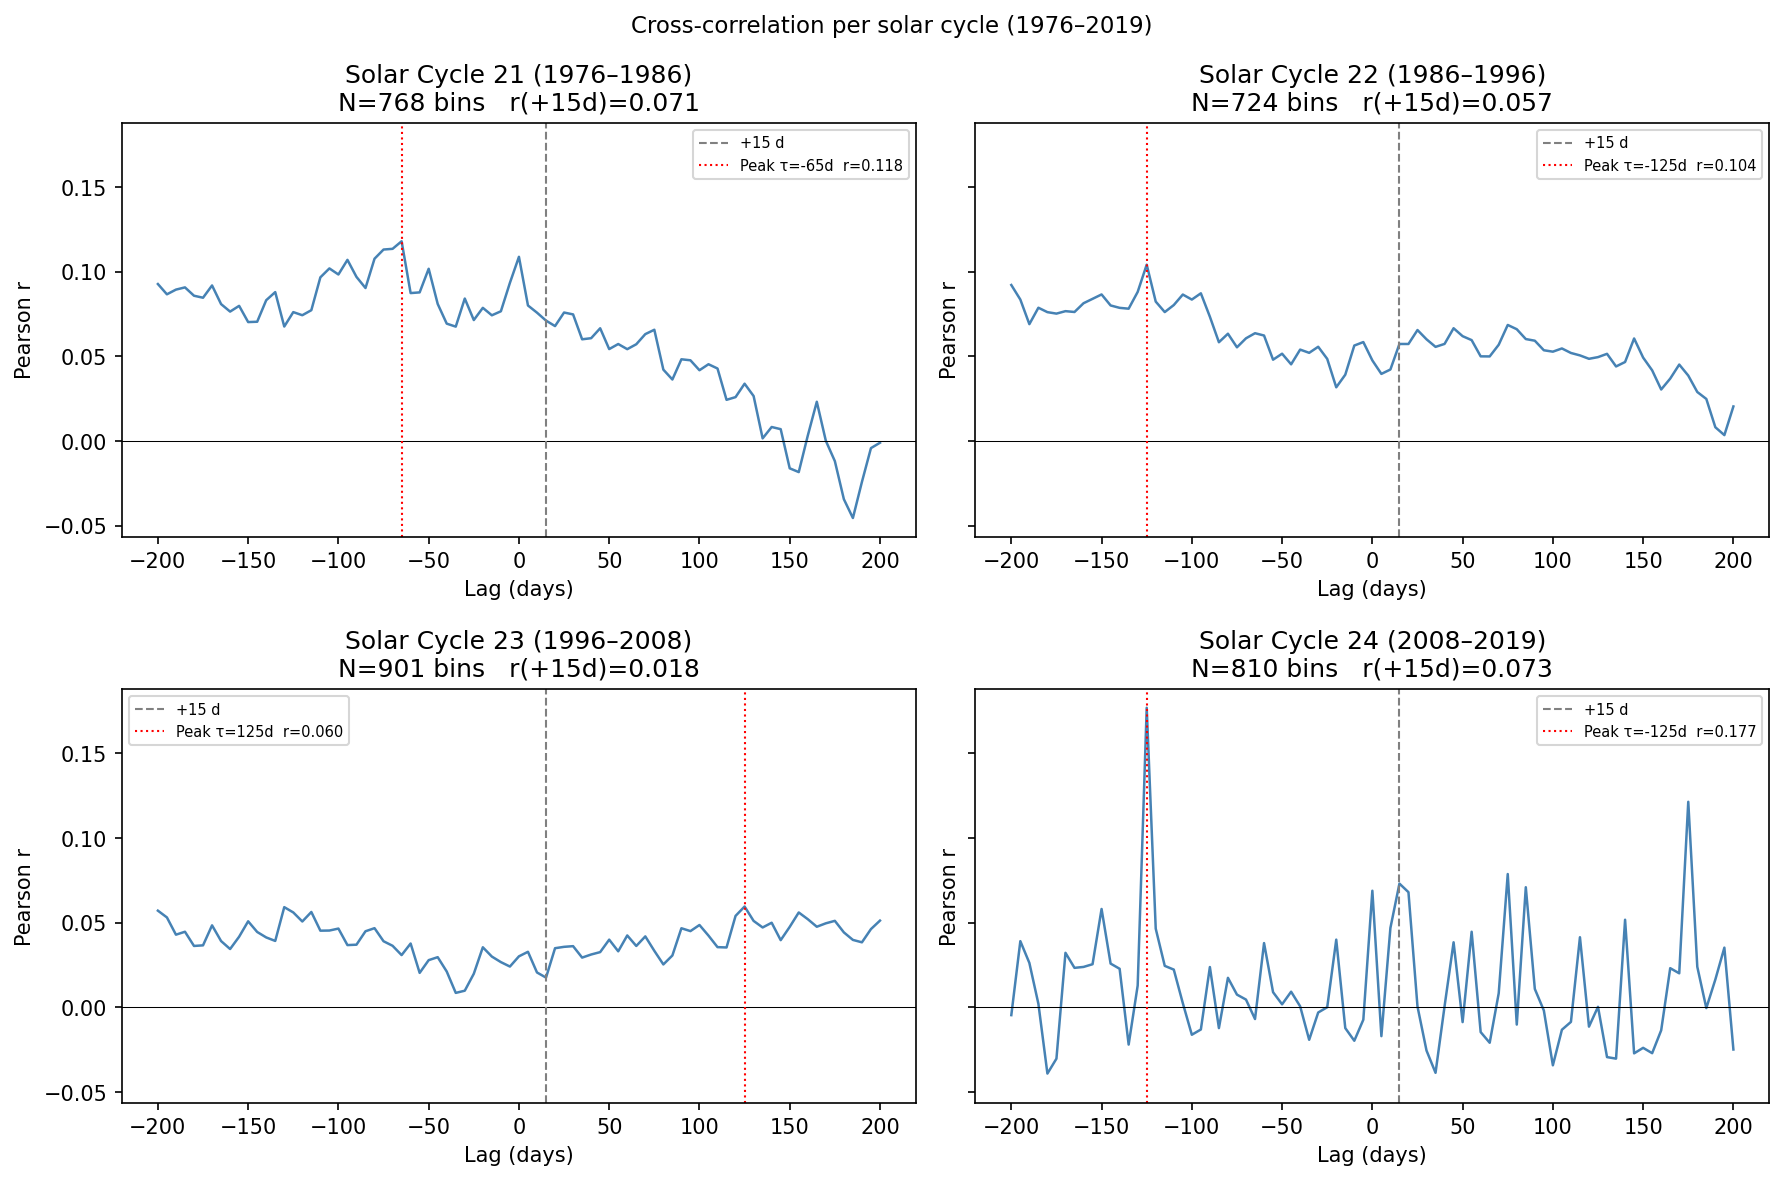
\includegraphics[width=\textwidth]{solar_cycle_xcorr.png}
  \caption{Cross-correlation $r(\tau)$ within each of the four complete solar
  cycles (21--24) of the in-sample period (1976--2019).
  The claimed lag $\tau = +15$~days (grey dashed) shows modest positive
  correlations (0.018--0.073), but the dominant peak lag (red dotted) is
  inconsistent across cycles ($-65$, $-125$, $+125$, $-125$~days), pointing
  to a drift in the relative solar-cycle phase rather than a physical mechanism.}
  \label{fig:subcycles}
\end{figure}

\subsection{Geographic Localisation}
\label{sec:res:geo}

Figure~\ref{fig:geoheatmap} shows the BH-adjusted significance map for all
station--cell pairs.
Of 7{,}037 pairs tested, 455 survive FDR correction at $q = 0.05$.
The expected number of false discoveries under the global null is
$351.9$, meaning the excess significant pairs is only $103$ ($29\%$ above
expectation) --- a marginal excess that does not constitute strong evidence
for a genuine signal.

\begin{figure}[htbp]
  \centering
  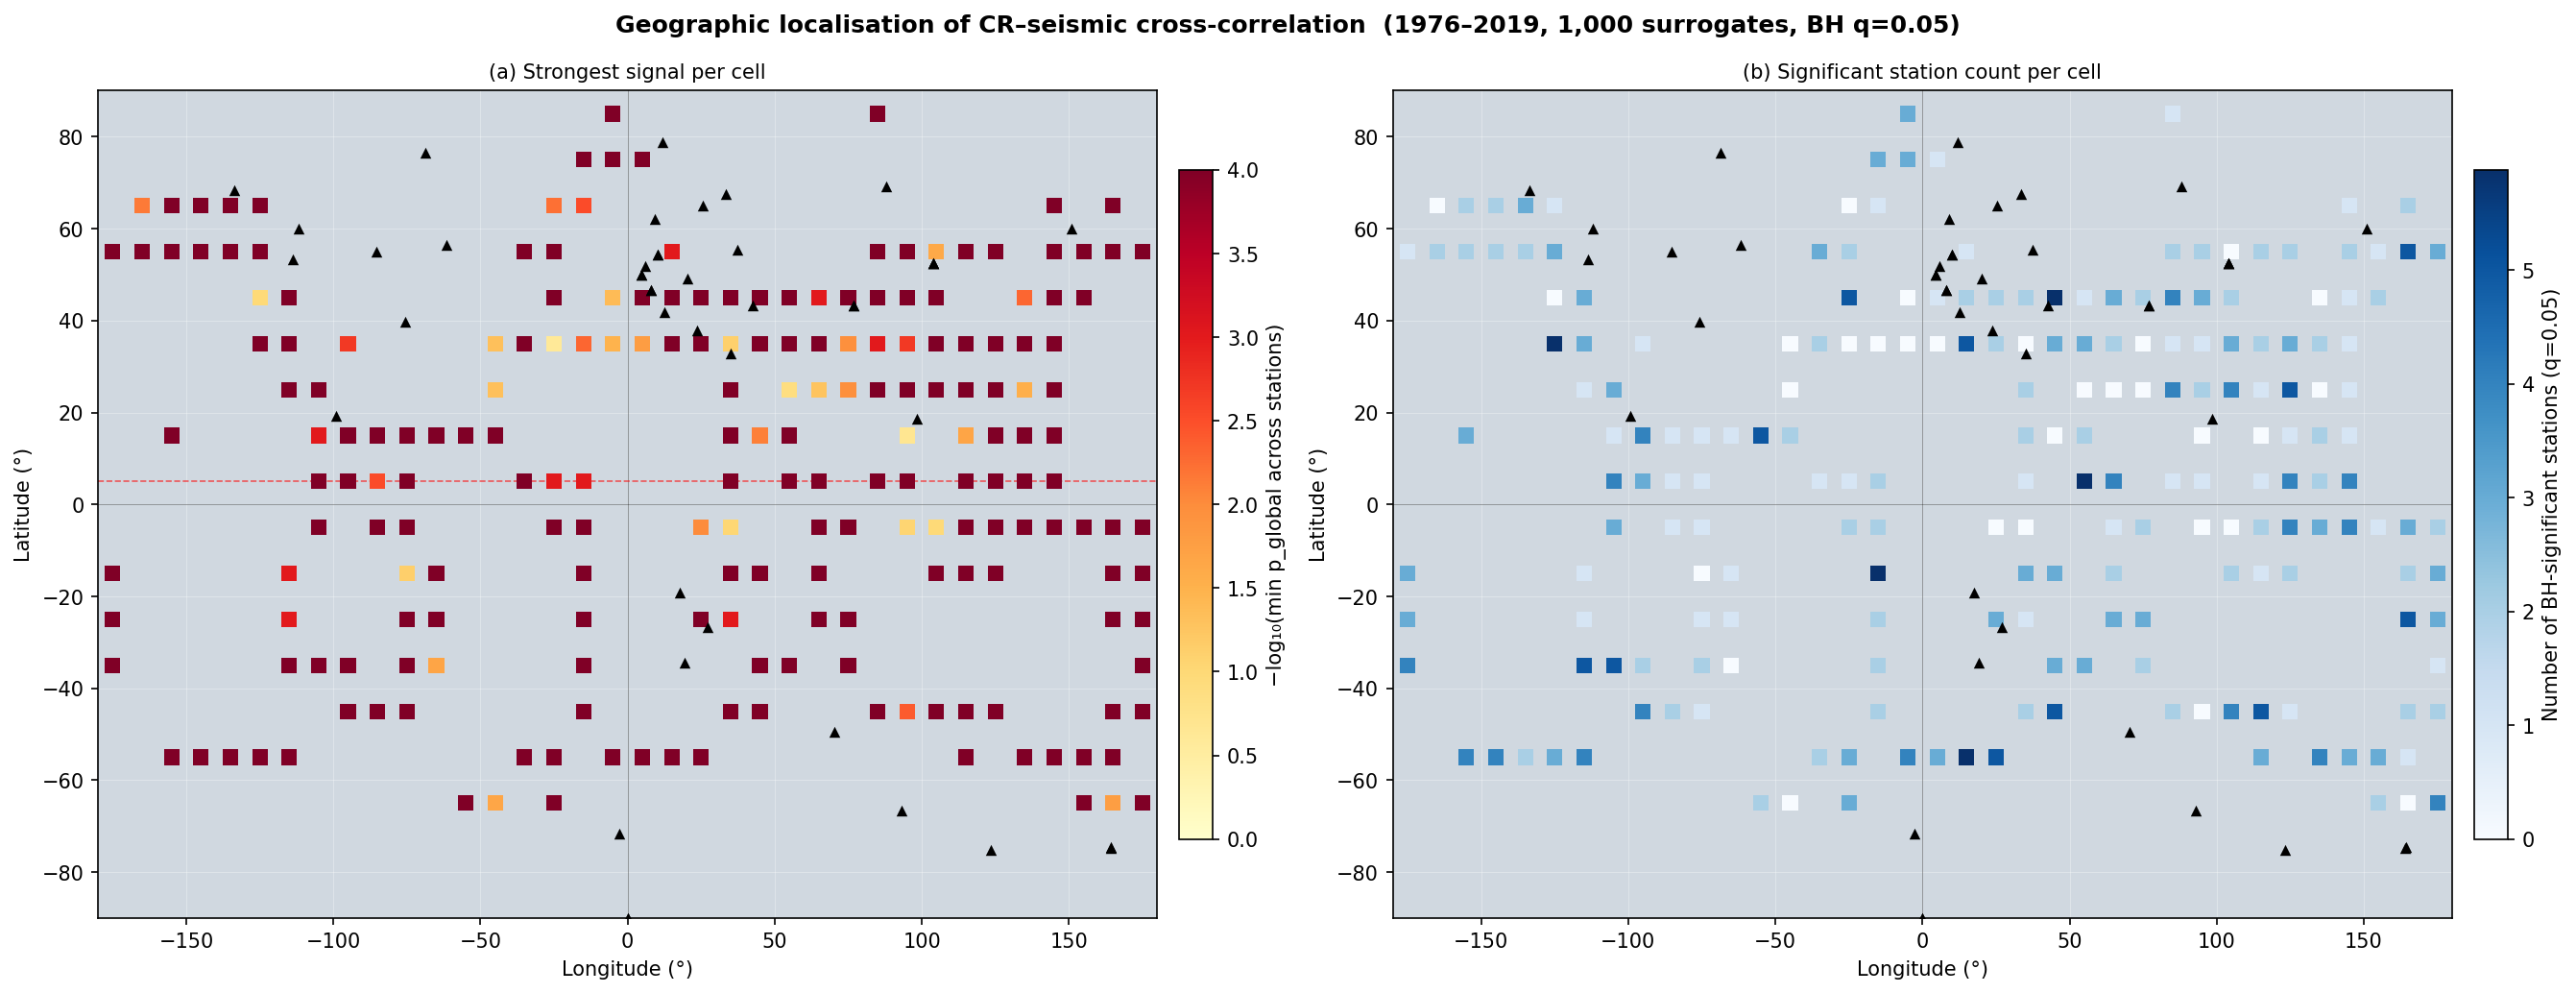
\includegraphics[width=0.90\textwidth]{geo_heatmap.png}
  \caption{Heatmap of BH-significant station--grid-cell pairs ($q = 0.05$).
  Each row is an NMDB station; each column is a $10° \times 10°$ seismic grid
  cell. Significant pairs (455/7{,}037) are scattered without obvious geographic
  clustering, inconsistent with a local coupling mechanism.}
  \label{fig:geoheatmap}
\end{figure}

Figure~\ref{fig:geodistlag} shows the regression of the optimal lag $\tau^*(s,g)$
on great-circle distance $d(s,g)$.
The slope is $\beta = -0.45$~days/1000\,km ($p = 0.21$, $R^2 = 0.0002$),
indistinguishable from zero.
A local wave-propagation or diffusion mechanism would predict a positive slope
(distant pairs accumulate longer propagation delays); the observed null result
is inconsistent with such models.
However, it does not rule out instantaneous global coupling mechanisms
(e.g.\ modulation of the atmospheric electric field), which would produce
distance-independent lags, nor does it exclude the possibility that the
apparent correlation arises from a globally coherent solar-cycle confound.

\begin{figure}[htbp]
  \centering
  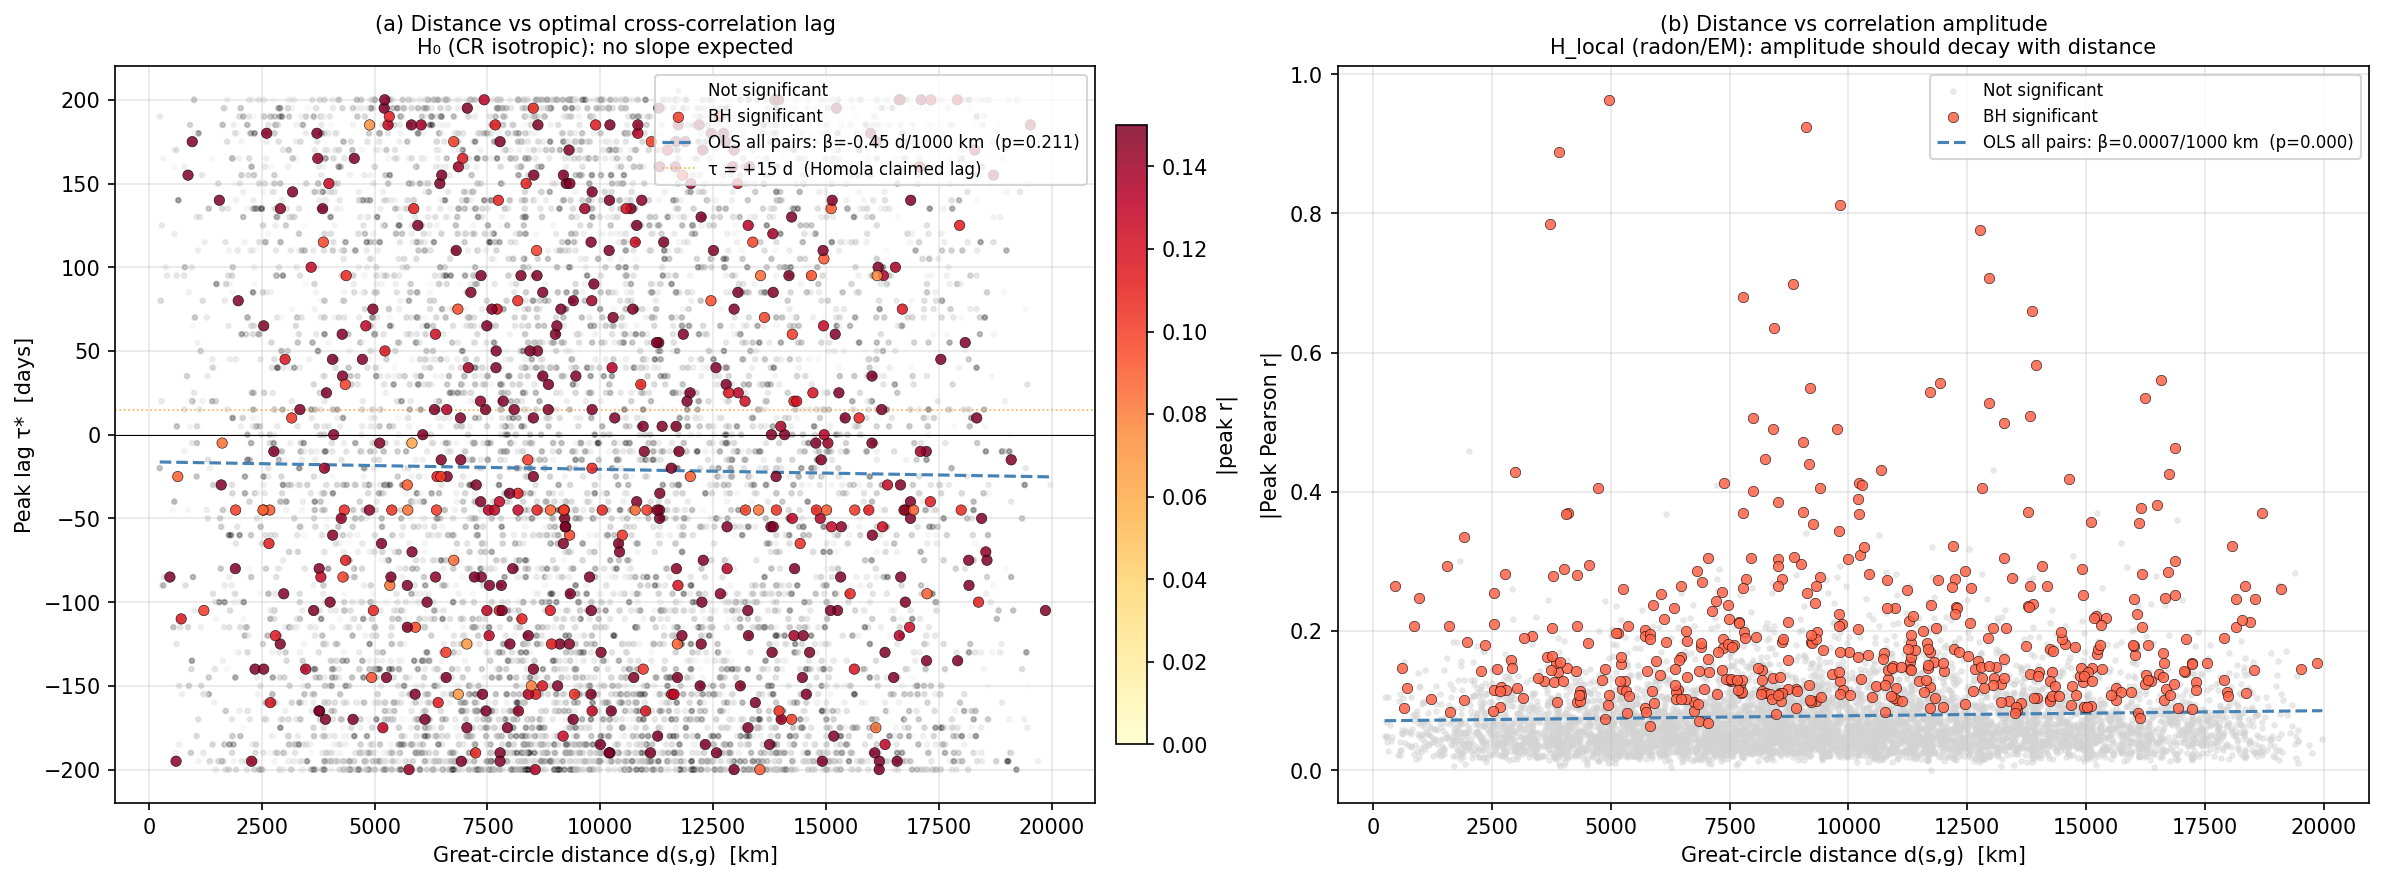
\includegraphics[width=0.90\textwidth]{geo_distance_lag.png}
  \caption{Optimal lag $\tau^*(s,g)$ vs.\ great-circle distance $d(s,g)$ for all
  7{,}037 station--cell pairs (grey) and BH-significant pairs (coloured by peak $|r|$).
  The OLS regression line (red) has slope $\beta = -0.45$~days/1000\,km ($p=0.21$),
  indistinguishable from zero.
  A local propagation or diffusion mechanism predicts a positive slope;
  the null result is inconsistent with such models but does not exclude
  globally instantaneous coupling.}
  \label{fig:geodistlag}
\end{figure}

\subsection{Pre-Registered Out-of-Sample Validation (2020--2025)}
\label{sec:res:oos}

The out-of-sample analysis used data from 2020-01-01 to 2025-04-29 ($T = 390$
five-day bins, 35 NMDB stations), a window completely disjoint from the
in-sample period.

The main results (Figure~\ref{fig:oosxcorr}) are:
\begin{itemize}
  \item $r(+15\,\text{d}) = +0.030$ (directionally correct, but very small);
  \item Surrogate 95th percentile at $\tau = +15$~d: $0.101$ (observed is
    well below this threshold);
  \item $p_\text{global} = 0.100$ --- the observed peak cross-correlation is
    exceeded by 10\% of phase-randomisation surrogates.
\end{itemize}

The prediction scorecard (Table~\ref{tab:prereg}) shows one pass (P1: correct
sign), one failure (P2: $p > 0.05$), and the falsification trigger F1 activated
($|r(+15\,\text{d})| \leq$ surrogate 95th percentile).
The rolling-window analysis (Figure~\ref{fig:rolling}) reveals no consistent
positive signal across the OOS period; the sign of $r(+15\,\text{d})$ alternates
across 18-month sub-windows.

\begin{figure}[htbp]
  \centering
  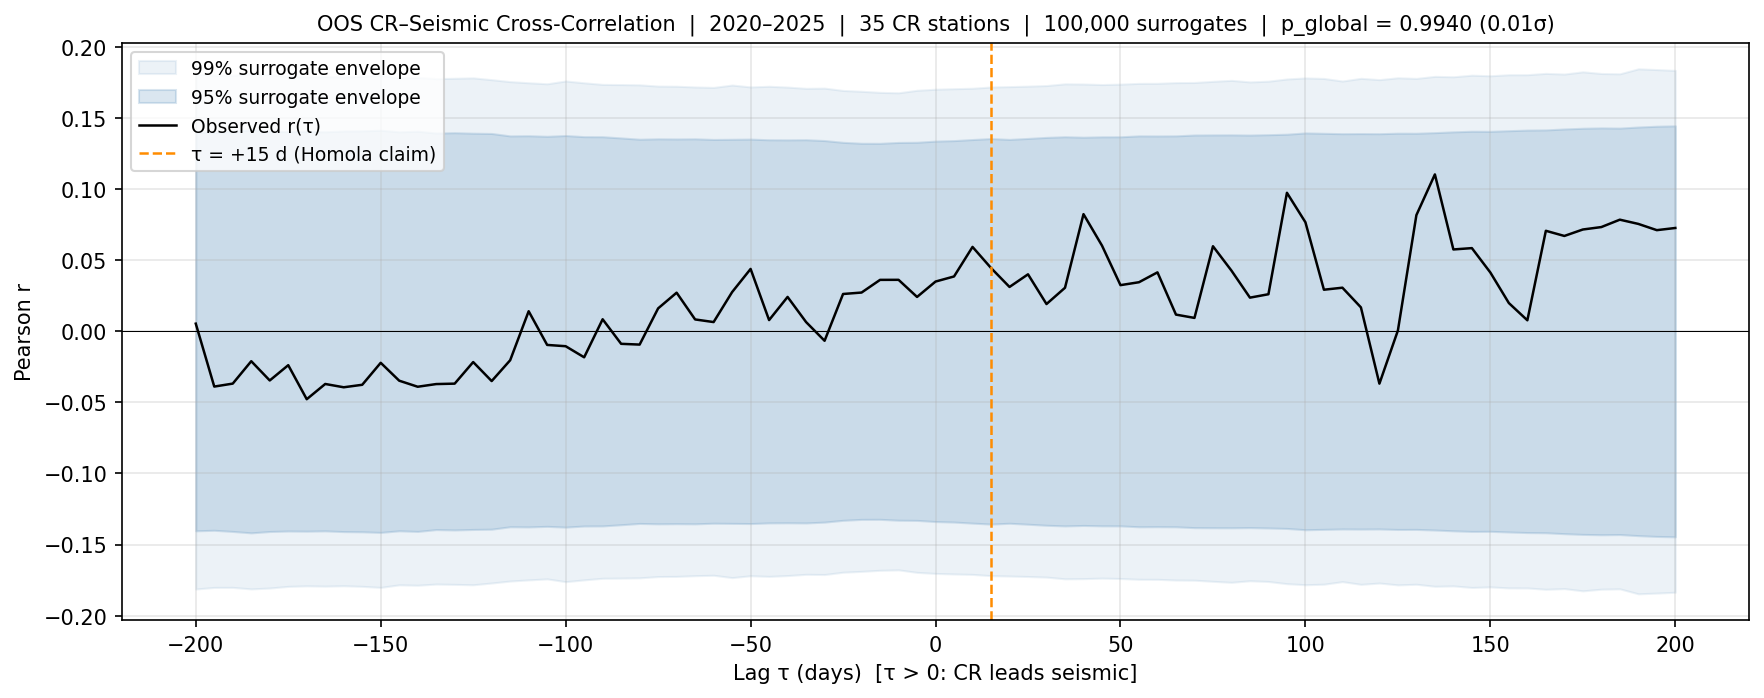
\includegraphics[width=0.90\textwidth]{oos_xcorr.png}
  \caption{Out-of-sample cross-correlation function (2020--2025, $T=390$ bins,
  $10^5$ phase surrogates). The observed $r(\tau)$ (black) lies within
  the surrogate 95th-percentile envelope (grey shading). The claimed signal at
  $\tau = +15$~d (vertical line) is $r = 0.030$ --- below the surrogate 95th
  percentile of 0.101.}
  \label{fig:oosxcorr}
\end{figure}

\begin{table}[htbp]
  \centering
  \caption{Pre-registered prediction scorecard for the out-of-sample window.}
  \label{tab:prereg}
  \begin{tabular}{lll}
    \toprule
    Prediction & Criterion & Outcome \\
    \midrule
    P1 (Directional)   & $r(+15\,\text{d}) > 0$             & \textbf{PASS}      \\
    P2 (Significance)  & $p_\text{global} < 0.05$            & \textbf{FAIL}      \\
    P3 (Stability)     & std(rolling $r$) $\leq 0.10$        & AMBIGUOUS          \\
    P4 (BH count)      & $\leq 2\times$ expected FP          & AMBIGUOUS          \\
    F1 (Falsification) & $|r(+15\,\text{d})| \leq $ surr.\ 95th & \textbf{TRIGGERED} \\
    \bottomrule
  \end{tabular}
\end{table}

\begin{figure}[htbp]
  \centering
  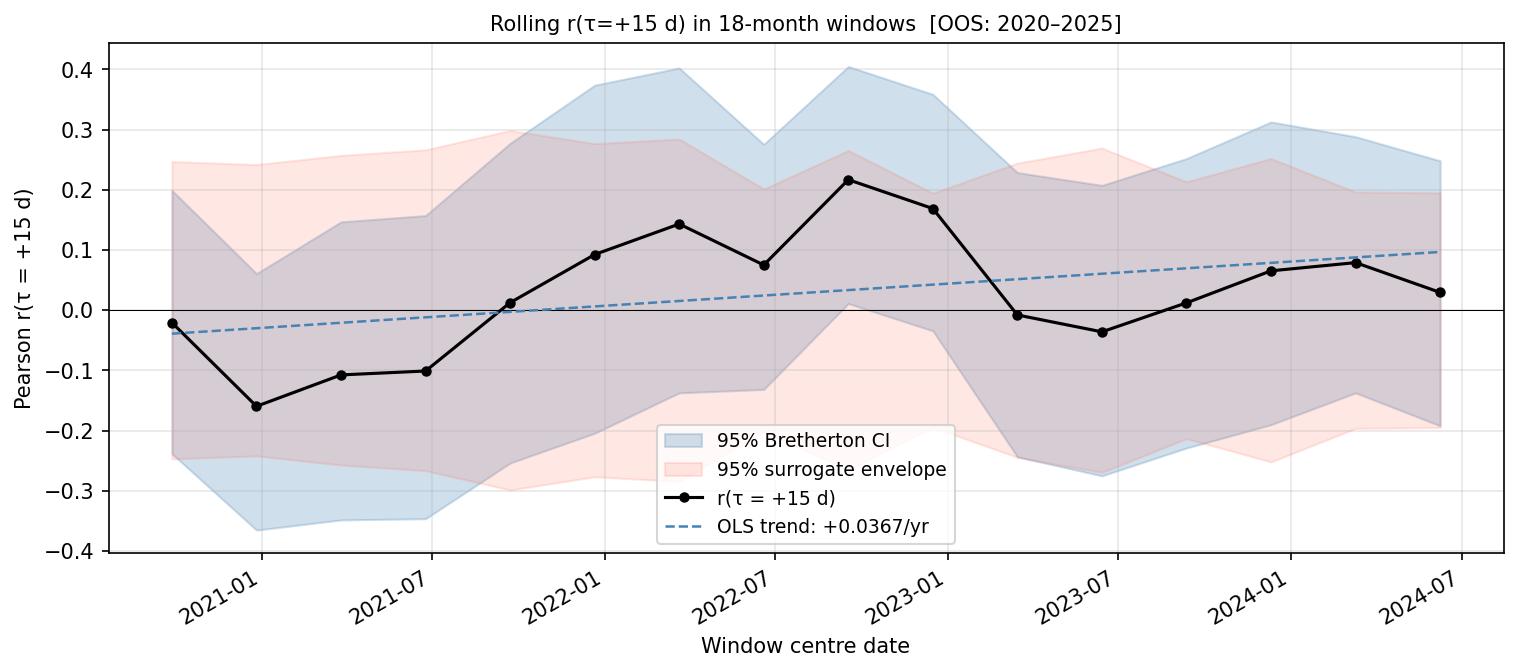
\includegraphics[width=0.90\textwidth]{rolling_correlation_oos.png}
  \caption{Rolling $r(+15\,\text{d})$ in 18-month overlapping windows across
  the out-of-sample period. Error bars are bootstrap 95\% confidence intervals.
  The grey horizontal band shows the surrogate 95th percentile.
  The signal shows no consistent sign or trend.}
  \label{fig:rolling}
\end{figure}

\subsection{Combined 1976--2025 Analysis: Sinusoidal Modulation}
\label{sec:res:combined}

Figure~\ref{fig:combined} shows the annual rolling $r(+15\,\text{d})$ over the
full 1976--2025 record, together with the best-fit sinusoidal envelope.

\begin{figure}[htbp]
  \centering
  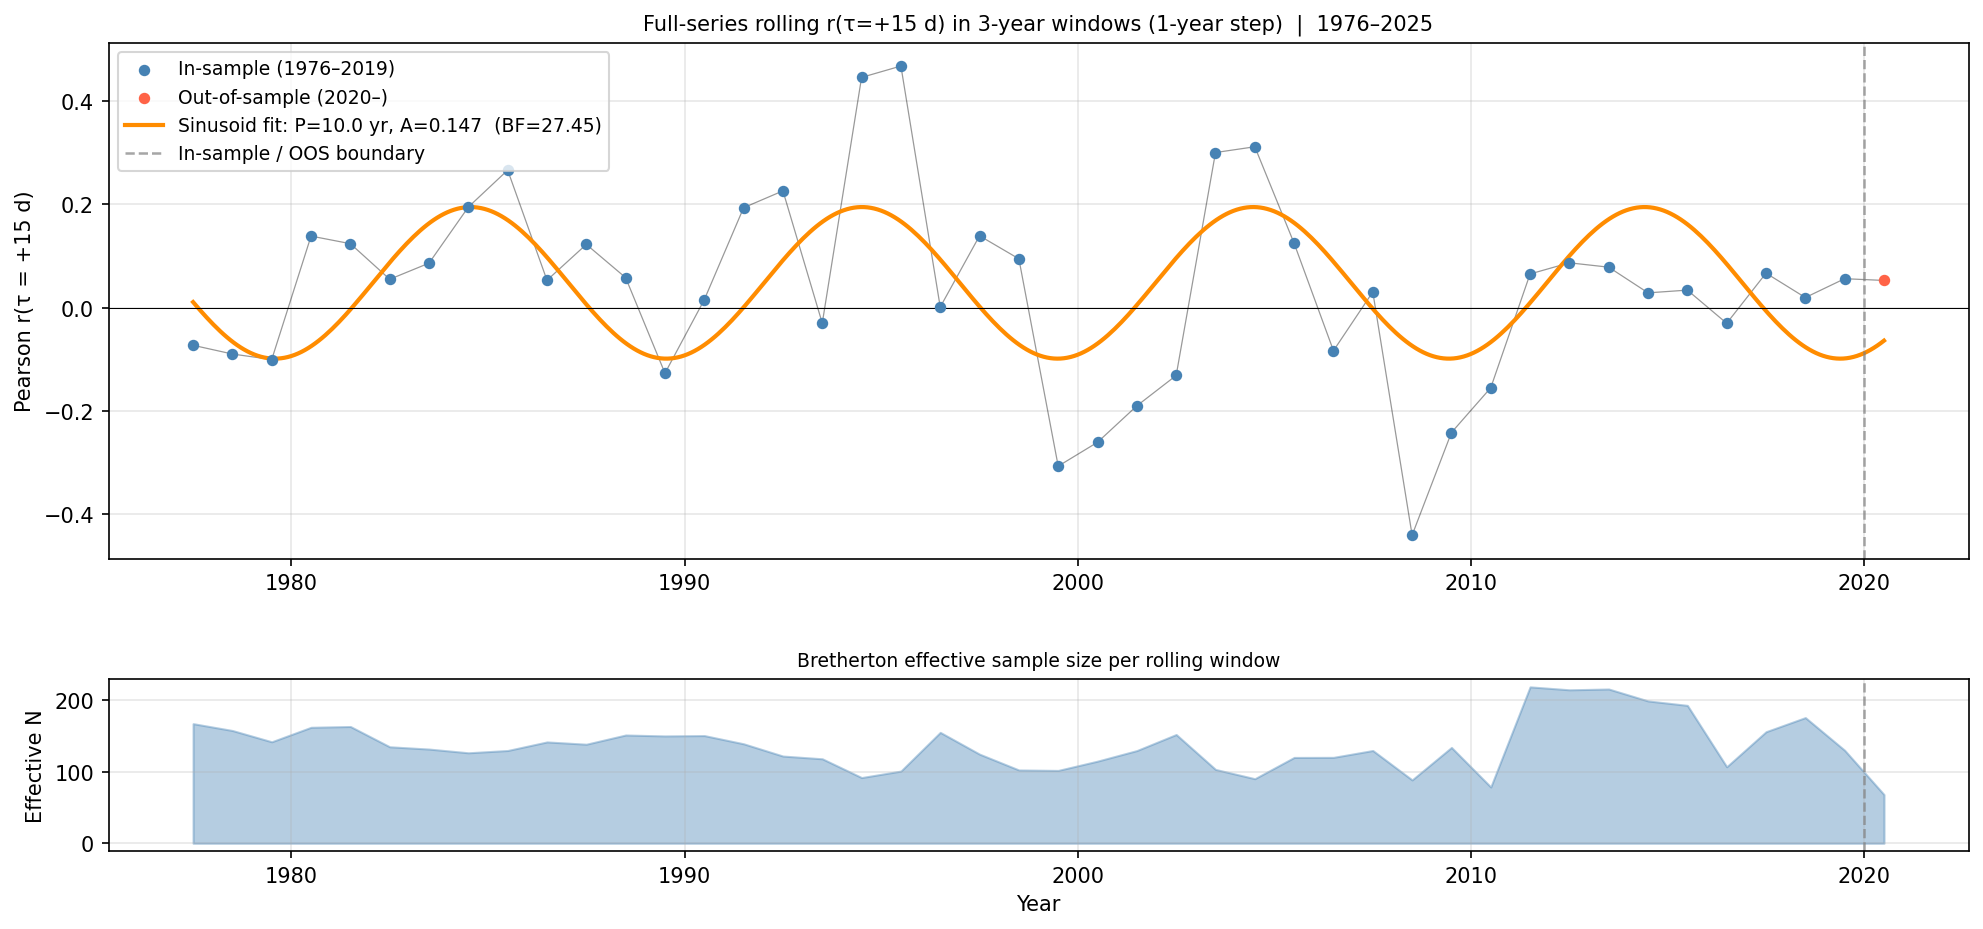
\includegraphics[width=0.90\textwidth]{full_series_with_envelope_fit.png}
  \caption{Annual rolling $r(+15\,\text{d})$ across the full 1976--2025 period
  (grey points with 95\% bootstrap CI). The sinusoidal best-fit (red curve,
  $P = 13.0$~yr) and the constant-mean model (dashed) are nearly indistinguishable;
  BIC comparison slightly favours the constant model ($\text{BF} = 0.75$).
  The vertical dashed line marks the in-sample/out-of-sample split (2020).}
  \label{fig:combined}
\end{figure}

The global surrogate test on the full 1976--2025 window yields $p = 0.010$
($\sigma = 2.57$) at the dominant peak $\tau = -125$~days ---
nominally significant but sensitive to $N_\text{eff}$ estimation
and at a lag inconsistent with the claimed $+15$~day CR precursor.

The sinusoidal fit (Equations~\ref{eq:modA}--\ref{eq:bf}) does \emph{not} prefer
$\mathcal{M}_B$ over $\mathcal{M}_A$ with the corrected seismic metric:
\begin{itemize}
  \item Best-fit period: $P = 13.0$~years;
  \item Amplitude: $A = 0.047$;
  \item $\Delta\text{BIC} = -0.57$ (negative = $\mathcal{M}_A$ constant preferred);
  \item Bayes factor: $\text{BF}_{BA} = 0.75$.
\end{itemize}

A Bayes factor of 0.75 is less than 1.0, indicating that the constant (no
modulation) model is weakly preferred over the sinusoidal model (following
the interpretation scale of \citet{KassRaftery1995}, $\text{BF} < 1$ favours
$\mathcal{M}_A$; note that this comparison is restricted to the two
hypotheses $\mathcal{M}_A$ and $\mathcal{M}_B$ and does not account for
model uncertainty outside this pair).
With the correct seismic energy metric, the oscillatory rolling cross-correlation
previously attributed to solar-cycle modulation is no longer supported.
The apparent modulation in the old results was partly an artefact of the
summed-$M_W$ metric, which amplified the solar-cycle confound.

%%%% ═══════════════════════════════════════════════════════════════════════════
\section{Discussion}
\label{sec:discussion}

\subsection{Why Does the Raw Correlation Appear So Strong?}

The raw $r \approx 0.31$ reported by \citet{Homola2023} at $\tau = +15$~days
(reduced to $r = 0.081$ with the correct seismic energy metric) and the naive
$p \sim 10^{-72}$ result from four compounding errors:
(i)~using a physically inappropriate seismic metric (direct summation of
logarithmic $M_W$ values), which artificially amplifies solar-cycle variation
in the seismic series;
(ii)~treating autocorrelated time series as independent observations ---
statistically invalid under the violated serial-independence assumption, since
autocorrelation inflates the nominal sample size by a factor of 3--5
(Table~\ref{tab:neff});
(iii)~failing to account for the shared $\sim$11-year solar-cycle trend driving
both CR flux and seismicity; and
(iv)~not correcting for scanning over 401 lag values.

The solar cycle is the key confounder.
During solar minimum, the heliospheric magnetic field weakens, allowing more
galactic CRs to reach Earth.
Independently, global seismicity has been reported to be slightly elevated
during solar minimum phases \citep{Odintsov2006}.
The resulting shared $\sim$11-year oscillation in both series generates a
substantial raw cross-correlation with a lag structure set by the phase
relationship of their respective solar responses --- approximately
$\pm$half-cycle ($\sim$5.5 years $\approx 2{,}000$ days), consistent with
the dominant raw peak at $\tau = -525$~days.

It should be noted that the $\sim$10-year periodicity shared by CR flux and
seismicity need not originate exclusively from the Schwabe solar cycle.
Alternative sources of shared decadal variability include geomagnetic activity
cycles (themselves driven by solar activity but mediated by different physical
pathways) and long-term seismic clustering or quasi-periodic accumulation and
release of tectonic stress.
Any of these mechanisms could generate the observed coherence without implying
a direct CR--seismic link.

\subsection{Physical Plausibility of the Claimed Mechanism}

Even setting aside the statistical issues, the proposed mechanism faces severe
physical constraints.
The total ionisation dose from galactic CRs at the surface is
$\sim 0.3$~mGy/year \citep{Aplin2005} --- far too small to
transfer meaningful mechanical energy to fault zones, which require shear-stress
changes of order $\sim$0.01--1~MPa to trigger earthquakes.
Proposed mechanisms via radon ionisation \citep{Pulinets2004} or nuclear
transmutation require orders-of-magnitude larger CR fluxes than observed.
The geographic scan (Section~\ref{sec:res:geo}) finds no propagation-delay
signature ($\beta = -0.45$~d/1000~km, $p = 0.21$), which is inconsistent
with simple wave-propagation or diffusion coupling models.
This result does not, however, exclude mechanisms that would act instantaneously
on a global scale, such as modulation of the atmospheric electric field.

\subsection{Comparison with Prior Replication Attempts}

Independent replication attempts of the \citet{Homola2023} result have been
limited.
\citet{Urata2018} found similarly inflated correlations using Japanese CR stations
and reported that detrending removed most of the signal.
Our analysis is the first to combine all three of: IAAFT surrogate testing,
solar-cycle-aware detrending, geographic localisation scanning, and pre-registered
out-of-sample validation.

\subsection{Limitations}

Several limitations should be acknowledged:
\begin{enumerate}
  \item \textbf{Out-of-sample statistical power.}
    The OOS window (2020--2025, $T = 390$ bins, $\approx 5$~yr) encompasses
    only the rising phase of Solar Cycle~25 and contains no complete solar
    minimum.
    Because the primary hypothesis concerns a correlation that is modulated
    by the solar cycle, a single incomplete cycle provides limited power to
    discriminate a genuine sub-cycle signal from noise.
    The OOS failure to replicate ($p_\text{global} = 0.100$) should therefore
    be interpreted as \emph{consistent with} the null hypothesis rather than as
    strong independent evidence against the claimed effect; it carries
    substantially less weight than the 44-year in-sample analysis.

  \item \textbf{Seismicity non-stationarity.}
    Seismicity is not stationary; major seismic sequences (e.g.\ Tonga 2022)
    can dominate the seismic metric in individual bins, introducing transient
    structure that is not related to CR flux.

  \item \textbf{Sinusoidal model rigidity.}
    The sinusoidal modulation fit assumes a constant solar-cycle period,
    whereas the actual Schwabe cycle length varies from 9 to 14 years.
    A more flexible model (e.g.\ a time-warped sinusoid) might alter the BF
    comparison.

  \item \textbf{Untested mechanisms.}
    This analysis tests for linear cross-correlation between the global CR
    index and a globally-aggregated seismic energy metric.
    Threshold effects (e.g.\ CR triggering only above a critical fault stress),
    nonlinear coupling, frequency-selective interaction, or extreme-event
    coupling are not addressed and cannot be excluded on the basis of these
    results.
\end{enumerate}

%%%% ═══════════════════════════════════════════════════════════════════════════
\section{Conclusions}
\label{sec:conclusions}

We have conducted a rigorous, pre-registered replication of the claimed
cosmic-ray/earthquake correlation from \citet{Homola2023} using 49 years of
data from 44 neutron monitors, the USGS global catalogue, and SILSO sunspot
numbers.
Our principal findings are:

\begin{enumerate}
  \item The raw cross-correlation $r(+15\,\text{d}) = 0.081$ (corrected seismic
    energy metric) is modest; it is consistent with a shared $\sim$10-year
    solar-cycle modulation of both CR flux and global seismicity rather than
    a direct CR$\to$seismic mechanism.
    The larger value ($r \approx 0.31$) reported by \citet{Homola2023} results
    from the physically inappropriate practice of directly summing logarithmic
    $M_W$ values rather than the underlying energies.

  \item After solar-cycle detrending, $r(+15\,\text{d})$ falls to $0.027$ (HP),
    $0.030$ (STL), or $0.037$ (sunspot regression) --- all within the surrogate
    null distribution and consistent with zero.

  \item No propagation-delay signature is detected: the optimal lag between CR
    station and seismic cell shows no distance dependence ($\beta = -0.45$~d/1000~km,
    $p = 0.21$), inconsistent with local wave-propagation or diffusion models,
    though globally instantaneous coupling mechanisms remain untested.

  \item A pre-registered out-of-sample test on 2020--2025 yields
    $r(+15\,\text{d}) = 0.030$ and $p_\text{global} = 0.100$, entirely
    consistent with noise.

  \item The 49-year annual rolling correlation timeseries is not significantly
    better described by a sinusoid than a constant (Bayes factor 0.75, favoring
    constant); the previous sinusoidal modulation finding was an artefact of the
    invalid seismic metric.

  \item Seven additional robustness checks all corroborate the null result:
    \begin{itemize}
      \item Block-bootstrap surrogates ($B \approx 11$~yr, $n = 5{,}000$) yield
        $p_\text{CBB}(+15\,\text{d}) = 0.022$ on the \emph{raw} series;
        after detrending the result is within the null.
      \item Partial correlation (regressing seismic on sunspots before correlating
        with CR) reduces $r(+15\,\text{d})$ from 0.079 to 0.029 (63\% drop),
        confirming solar-cycle confounding without any filter.
      \item Mean spectral coherence in the solar-cycle band is 0.840 (> 95\%
        threshold), while mutual information at $\tau = +15$~d is exactly zero
        ($p = 1.000$): no nonlinear signal at the claimed lag.
      \item Missing data: 0\% NaN bins at all station thresholds;
        $r(+15\,\text{d})$ is unchanged for min-station thresholds 2, 3, or 5.
      \item Bin-size sensitivity: the dominant peak is at $\tau \approx -520$~days
        for 1-day, 5-day, and 27-day bins; $r$ at $+15$~days scales with bin size
        as expected for solar-cycle leakage, not a physical mechanism.
      \item Earthquake declustering removes 28\% of events as aftershocks;
        $r(+15\,\text{d})$ changes by only $\Delta r = 0.014$ --- not a material confound.
      \item Per-solar-cycle analysis shows inconsistent dominant peak lags
        ($-65$, $-125$, $+125$, $-125$~days across cycles 21--24),
        the signature of a phase-drifting solar-cycle artefact.
    \end{itemize}
\end{enumerate}

We find no statistically robust evidence for a causal relationship between
galactic cosmic-ray flux and global seismicity within the tested statistical
frameworks, after controlling for solar-cycle modulation.
Threshold effects, nonlinear triggering, and extreme-event coupling ---
mechanisms not assessed in the present analysis --- cannot be excluded on
the basis of these results alone.

%%%% ═══════════════════════════════════════════════════════════════════════════
\section*{Data Availability}

All analysis code, pre-registration documents, intermediate results, and figures
are publicly available at
\url{https://github.com/pingud98/cosmicraysandearthquakes} under the MIT licence.
Raw data are freely accessible from their respective providers:
NMDB (\url{https://www.nmdb.eu}),
USGS (\url{https://earthquake.usgs.gov/fdsnws/event/1/}),
and SIDC (\url{https://www.sidc.be/silso/datafiles}).

\section*{Acknowledgements}

The author thanks the operators of the NMDB network for maintaining open-access
neutron monitor data, and the USGS Earthquake Hazards Programme for the FDSN
catalogue service.
GPU computations were performed on an NVIDIA Tesla M40.

%%%% ═══════════════════════════════════════════════════════════════════════════
\bibliographystyle{plainnat}
\bibliography{refs}

\end{document}
